\documentclass[11pt]{article}
\usepackage[textwidth=18.0cm, textheight=23.0cm, top=2.0cm]{geometry}
\usepackage{pst-all}
\usepackage{amssymb}
\usepackage{tikz}
\usepackage{underscore}\begin{document}
\pagestyle{empty}


ClassName: \underline{\textbf{Class_05.2bp-22}}
\par
BinSize: \underline{\textbf{100 × 100}}
\par
ReduceSize: \underline{\textbf{100 × 100}}
\par
TypeNum: \underline{\textbf{60}}
\par
Num: \underline{\textbf{60}}
\par
OutS: \underline{\textbf{190000}}
\par
InS: \underline{\textbf{154680}}
\par
Rate: \underline{\textbf{0.814}}
\par
UB: \underline{\textbf{19}}
\par
LB0: \underline{\textbf{19}}
\par
LB: \underline{\textbf{19}}
\par
LBWithCut: \underline{\textbf{19}}
\par
NodeCut: \underline{\textbf{0}}
\par
ExtendedNodeCnt: \underline{\textbf{1}}
\par
GenNodeCnt: \underline{\textbf{1}}
\par
PrimalNode: \underline{\textbf{0}}
\par
ColumnCount: \underline{\textbf{19}}
\par
TotalCutCount: \underline{\textbf{0}}
\par
RootCutCount: \underline{\textbf{0}}
\par
LPSolverCnt: \underline{\textbf{1}}
\par
PricingSolverCnt: \underline{\textbf{0}}
\par
BranchAndBoundNum: \underline{\textbf{1}}
\par
isOpt: \underline{\textbf{true}}
\par
TimeOnInitSolution: \underline{\textbf{0.340 s}}
\par
TimeOnPrimal: \underline{\textbf{0.000 s}}
\par
TimeOnPricing: \underline{\textbf{0.000 s}}
\par
TimeOnRmp: \underline{\textbf{0.063 s}}
\par
TotalTime: \underline{\textbf{0.481 s}}
\par
\newpage


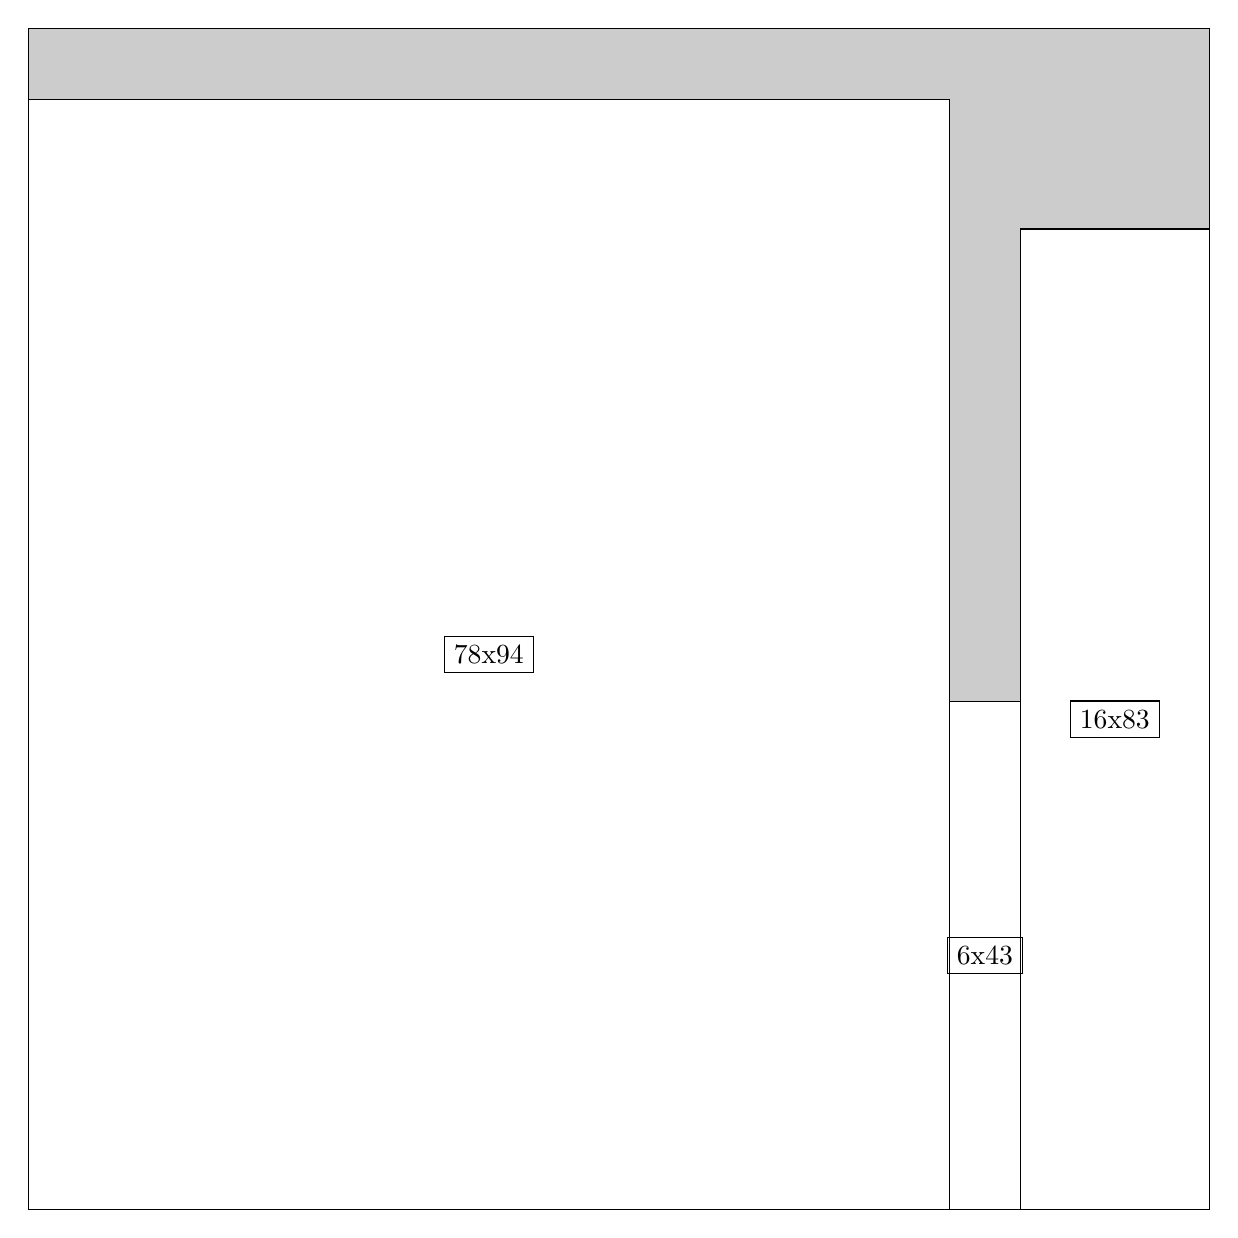
\begin{tikzpicture}[shorten >=1pt,scale=1.0,every node/.style={scale=1.0},->]
\tikzstyle{vertex}=[circle,fill=black!25,minimum size=14pt,inner sep=0pt]
\filldraw[fill=gray!40!white, draw=black] (0,0) rectangle (15.0,15.0);
\foreach \name/\x/\y/\w/\h in {78x94/0.0/0.0/11.7/14.1,16x83/12.6/0.0/2.4/12.45,6x43/11.7/0.0/0.8999999999999999/6.45}
\filldraw[fill=white!40!white, draw=black] (\x,\y) rectangle node[draw] (\name) {\name} ++(\w,\h);
\end{tikzpicture}


w =78 , h =94 , x =0 , y =0 , v =7332
\par
w =16 , h =83 , x =84 , y =0 , v =1328
\par
w =6 , h =43 , x =78 , y =0 , v =258
\par
\newpage


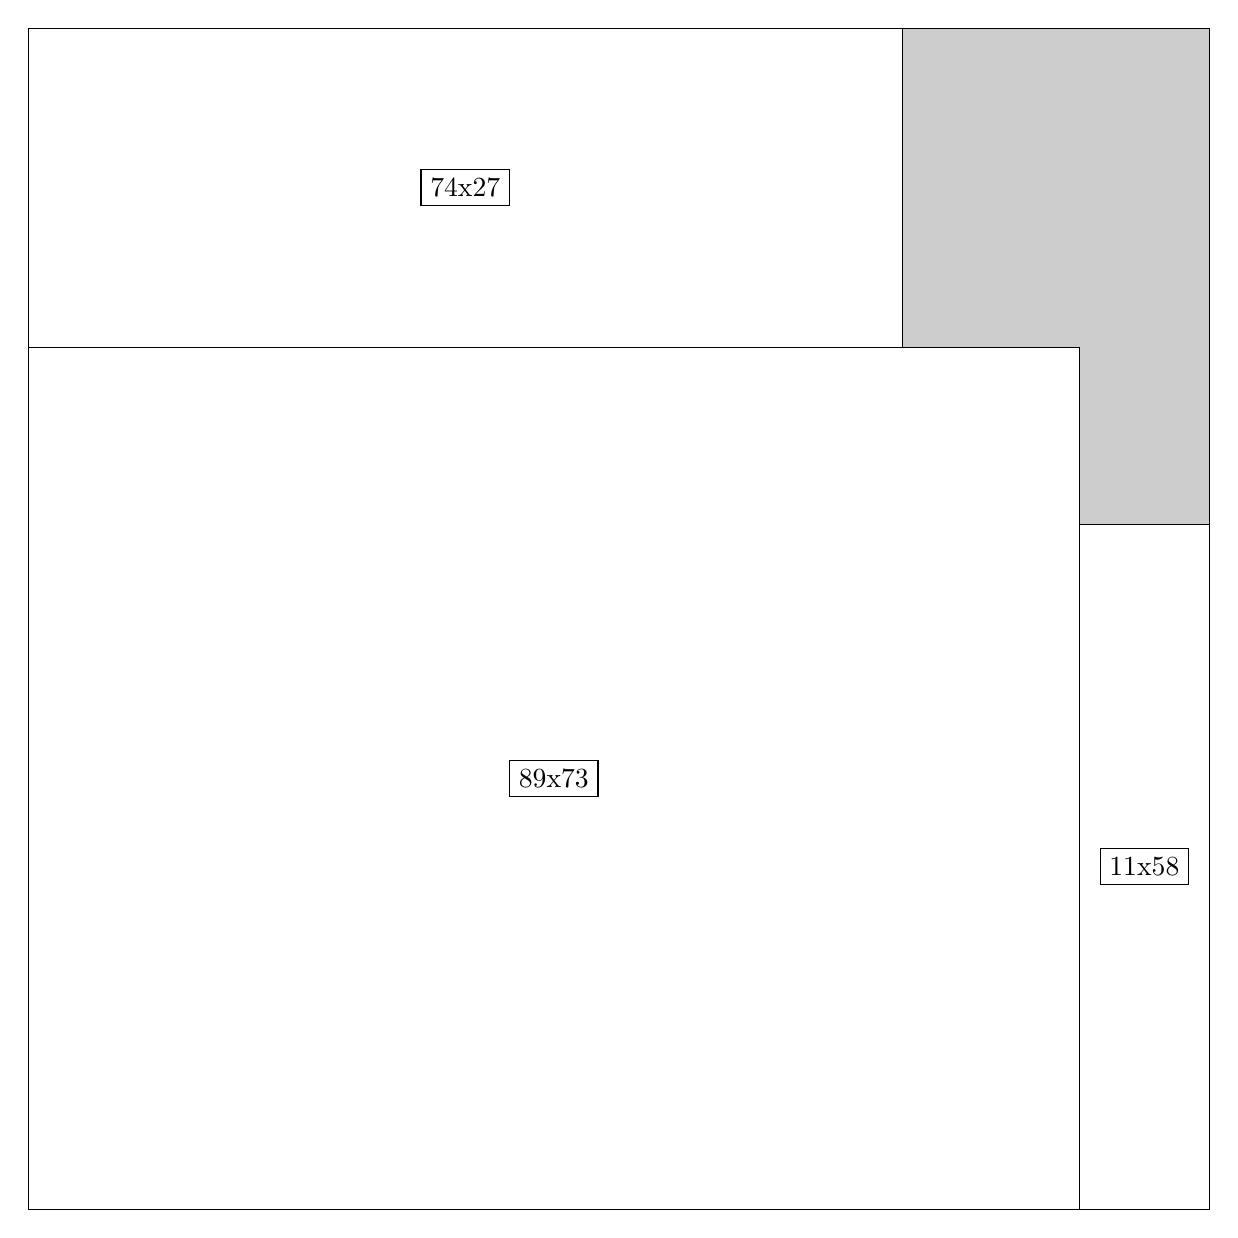
\begin{tikzpicture}[shorten >=1pt,scale=1.0,every node/.style={scale=1.0},->]
\tikzstyle{vertex}=[circle,fill=black!25,minimum size=14pt,inner sep=0pt]
\filldraw[fill=gray!40!white, draw=black] (0,0) rectangle (15.0,15.0);
\foreach \name/\x/\y/\w/\h in {89x73/0.0/0.0/13.35/10.95,74x27/0.0/10.95/11.1/4.05,11x58/13.35/0.0/1.65/8.7}
\filldraw[fill=white!40!white, draw=black] (\x,\y) rectangle node[draw] (\name) {\name} ++(\w,\h);
\end{tikzpicture}


w =89 , h =73 , x =0 , y =0 , v =6497
\par
w =74 , h =27 , x =0 , y =73 , v =1998
\par
w =11 , h =58 , x =89 , y =0 , v =638
\par
\newpage


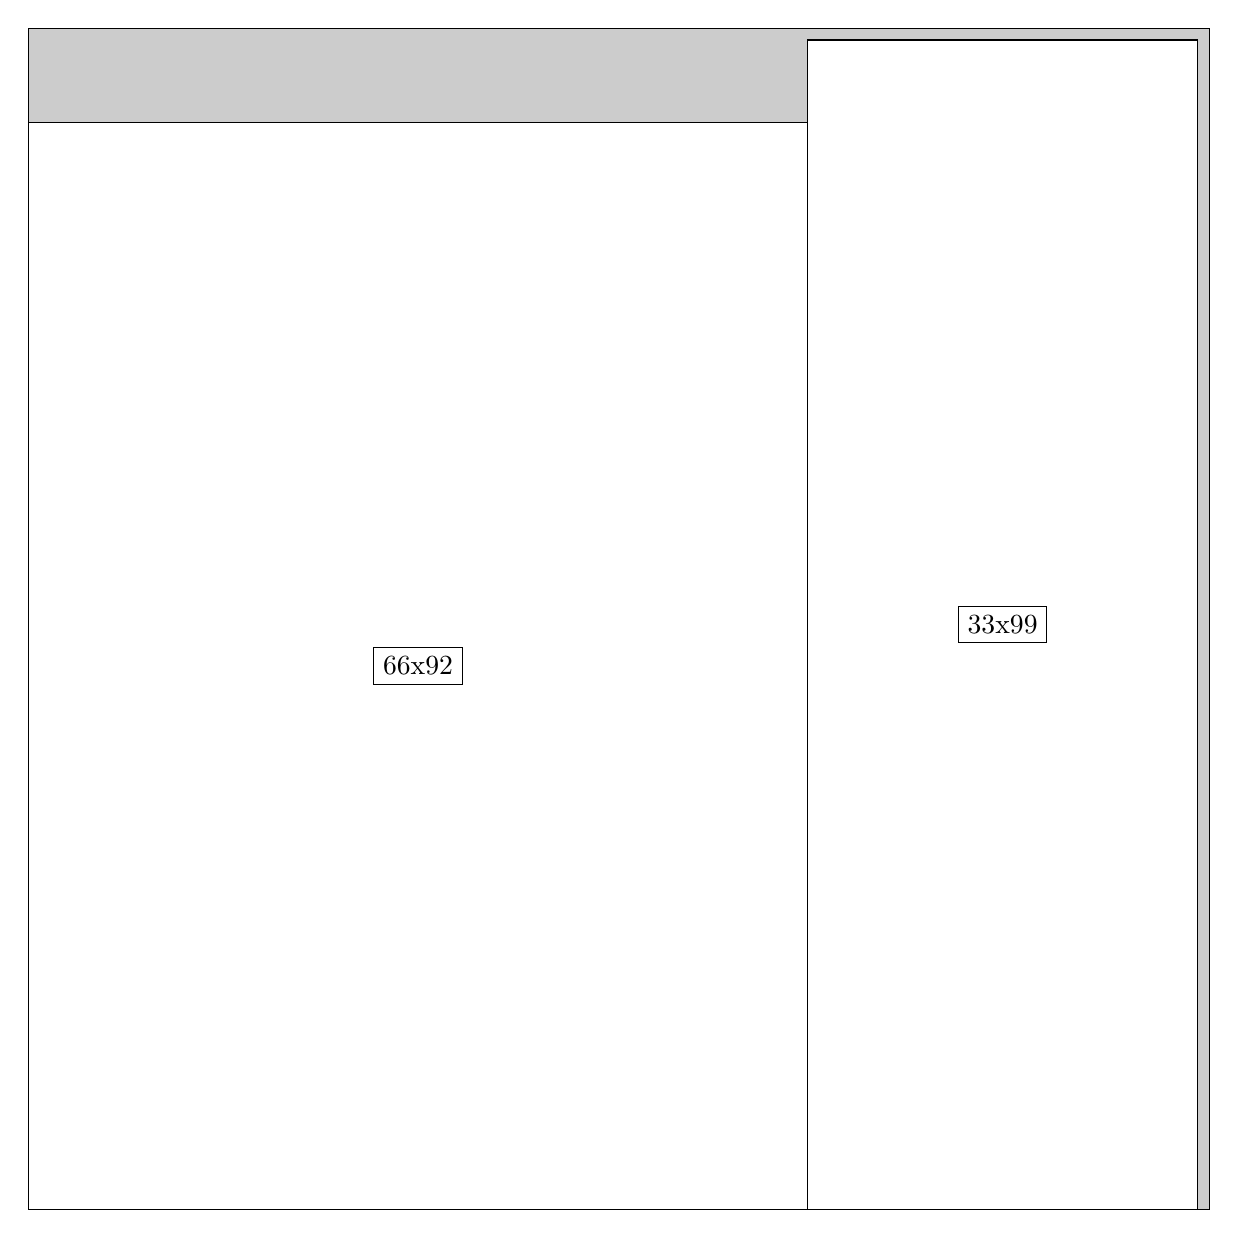
\begin{tikzpicture}[shorten >=1pt,scale=1.0,every node/.style={scale=1.0},->]
\tikzstyle{vertex}=[circle,fill=black!25,minimum size=14pt,inner sep=0pt]
\filldraw[fill=gray!40!white, draw=black] (0,0) rectangle (15.0,15.0);
\foreach \name/\x/\y/\w/\h in {66x92/0.0/0.0/9.9/13.799999999999999,33x99/9.9/0.0/4.95/14.85}
\filldraw[fill=white!40!white, draw=black] (\x,\y) rectangle node[draw] (\name) {\name} ++(\w,\h);
\end{tikzpicture}


w =66 , h =92 , x =0 , y =0 , v =6072
\par
w =33 , h =99 , x =66 , y =0 , v =3267
\par
\newpage


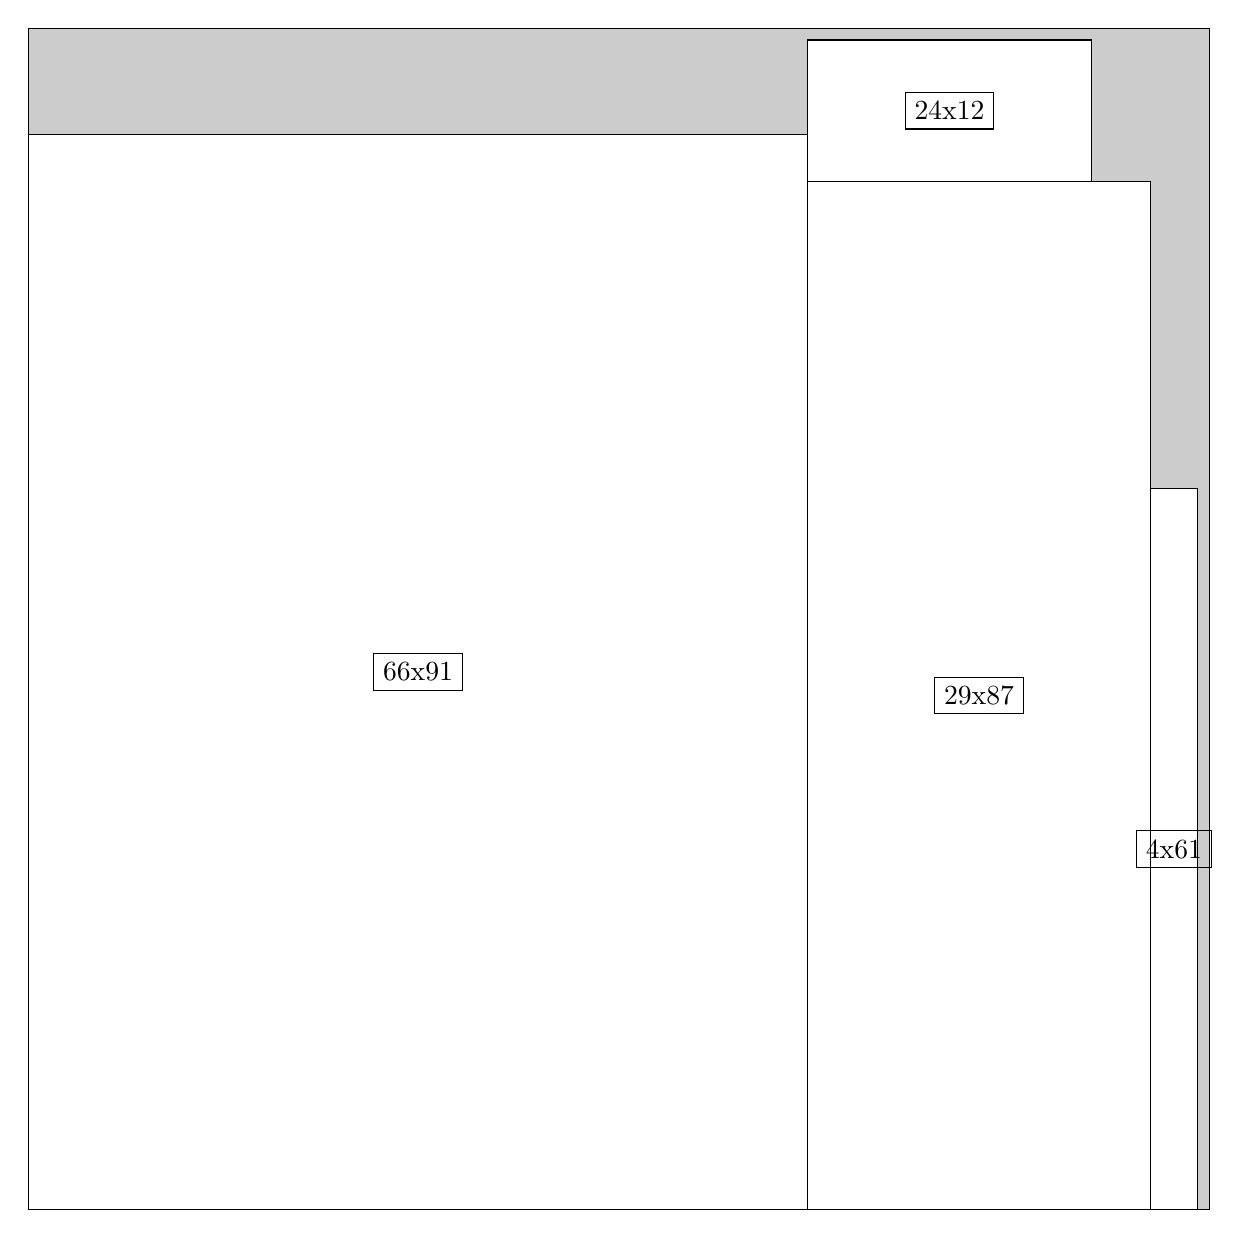
\begin{tikzpicture}[shorten >=1pt,scale=1.0,every node/.style={scale=1.0},->]
\tikzstyle{vertex}=[circle,fill=black!25,minimum size=14pt,inner sep=0pt]
\filldraw[fill=gray!40!white, draw=black] (0,0) rectangle (15.0,15.0);
\foreach \name/\x/\y/\w/\h in {66x91/0.0/0.0/9.9/13.65,29x87/9.9/0.0/4.35/13.049999999999999,24x12/9.9/13.049999999999999/3.5999999999999996/1.7999999999999998,4x61/14.25/0.0/0.6/9.15}
\filldraw[fill=white!40!white, draw=black] (\x,\y) rectangle node[draw] (\name) {\name} ++(\w,\h);
\end{tikzpicture}


w =66 , h =91 , x =0 , y =0 , v =6006
\par
w =29 , h =87 , x =66 , y =0 , v =2523
\par
w =24 , h =12 , x =66 , y =87 , v =288
\par
w =4 , h =61 , x =95 , y =0 , v =244
\par
\newpage


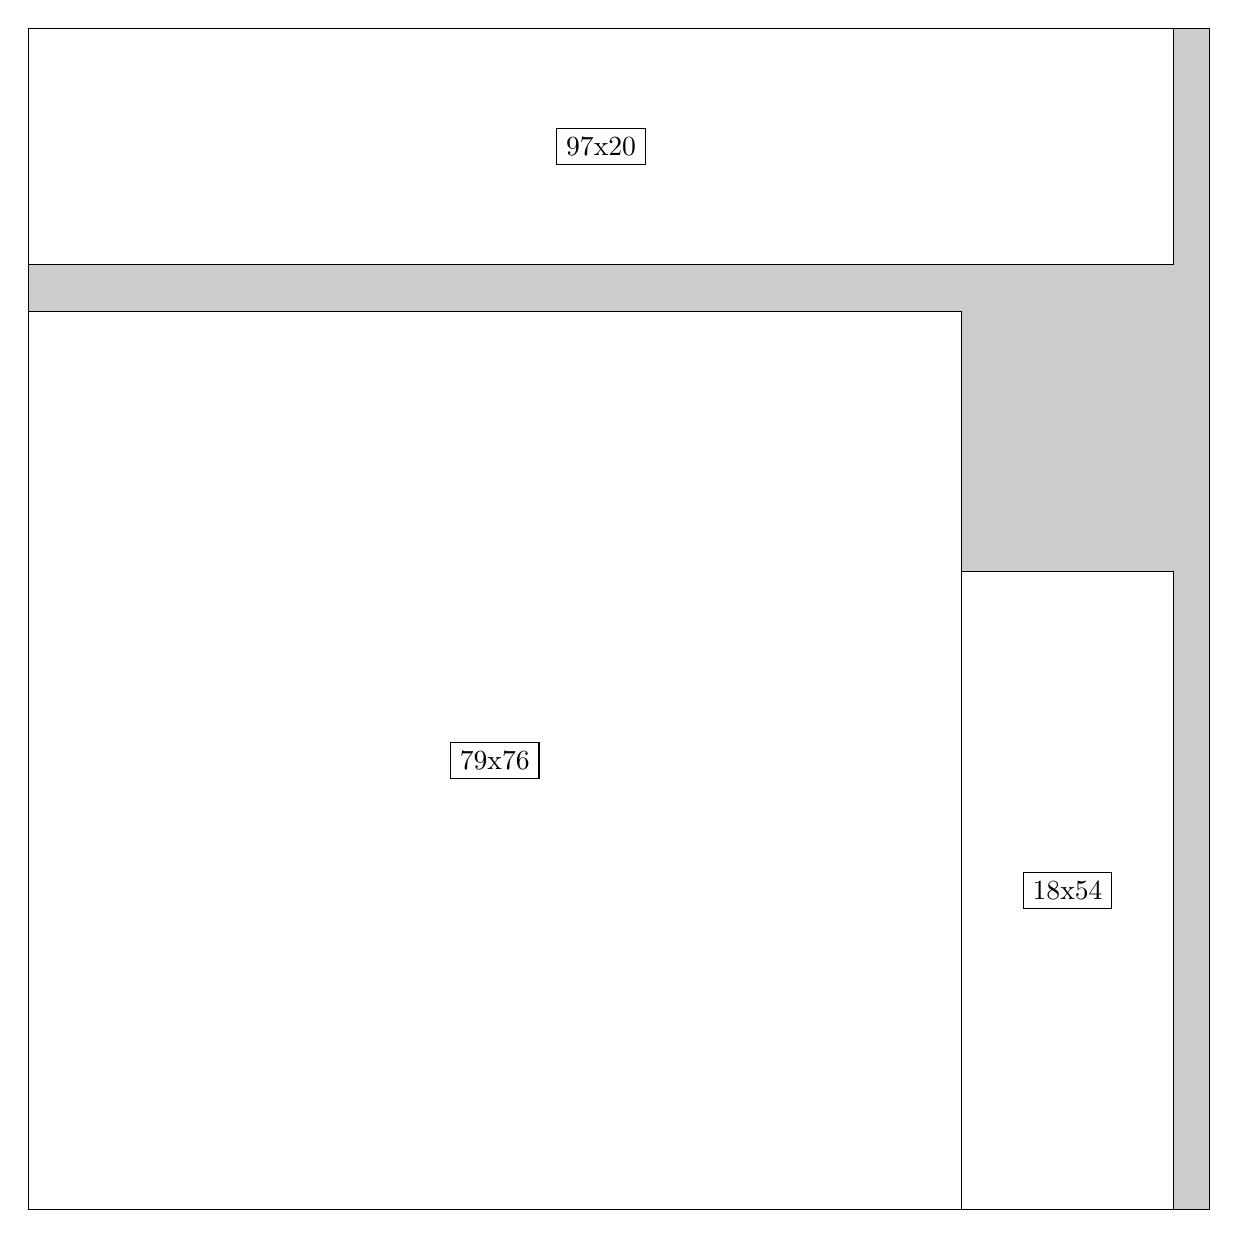
\begin{tikzpicture}[shorten >=1pt,scale=1.0,every node/.style={scale=1.0},->]
\tikzstyle{vertex}=[circle,fill=black!25,minimum size=14pt,inner sep=0pt]
\filldraw[fill=gray!40!white, draw=black] (0,0) rectangle (15.0,15.0);
\foreach \name/\x/\y/\w/\h in {79x76/0.0/0.0/11.85/11.4,97x20/0.0/12.0/14.549999999999999/3.0,18x54/11.85/0.0/2.6999999999999997/8.1}
\filldraw[fill=white!40!white, draw=black] (\x,\y) rectangle node[draw] (\name) {\name} ++(\w,\h);
\end{tikzpicture}


w =79 , h =76 , x =0 , y =0 , v =6004
\par
w =97 , h =20 , x =0 , y =80 , v =1940
\par
w =18 , h =54 , x =79 , y =0 , v =972
\par
\newpage


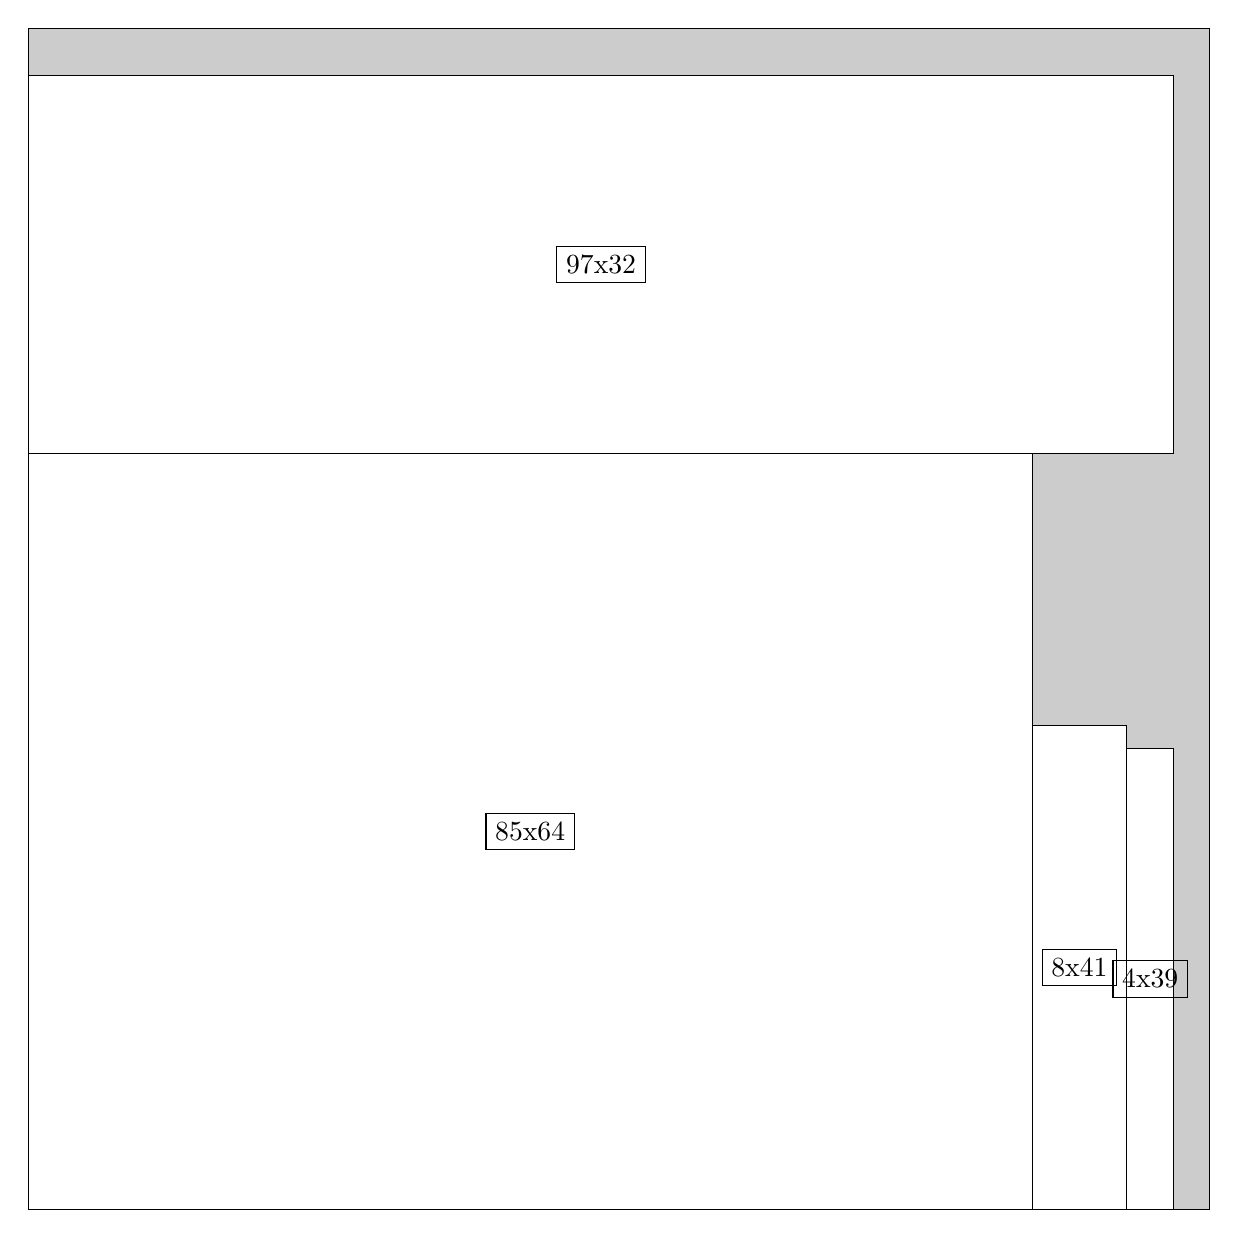
\begin{tikzpicture}[shorten >=1pt,scale=1.0,every node/.style={scale=1.0},->]
\tikzstyle{vertex}=[circle,fill=black!25,minimum size=14pt,inner sep=0pt]
\filldraw[fill=gray!40!white, draw=black] (0,0) rectangle (15.0,15.0);
\foreach \name/\x/\y/\w/\h in {85x64/0.0/0.0/12.75/9.6,97x32/0.0/9.6/14.549999999999999/4.8,8x41/12.75/0.0/1.2/6.1499999999999995,4x39/13.95/0.0/0.6/5.85}
\filldraw[fill=white!40!white, draw=black] (\x,\y) rectangle node[draw] (\name) {\name} ++(\w,\h);
\end{tikzpicture}


w =85 , h =64 , x =0 , y =0 , v =5440
\par
w =97 , h =32 , x =0 , y =64 , v =3104
\par
w =8 , h =41 , x =85 , y =0 , v =328
\par
w =4 , h =39 , x =93 , y =0 , v =156
\par
\newpage


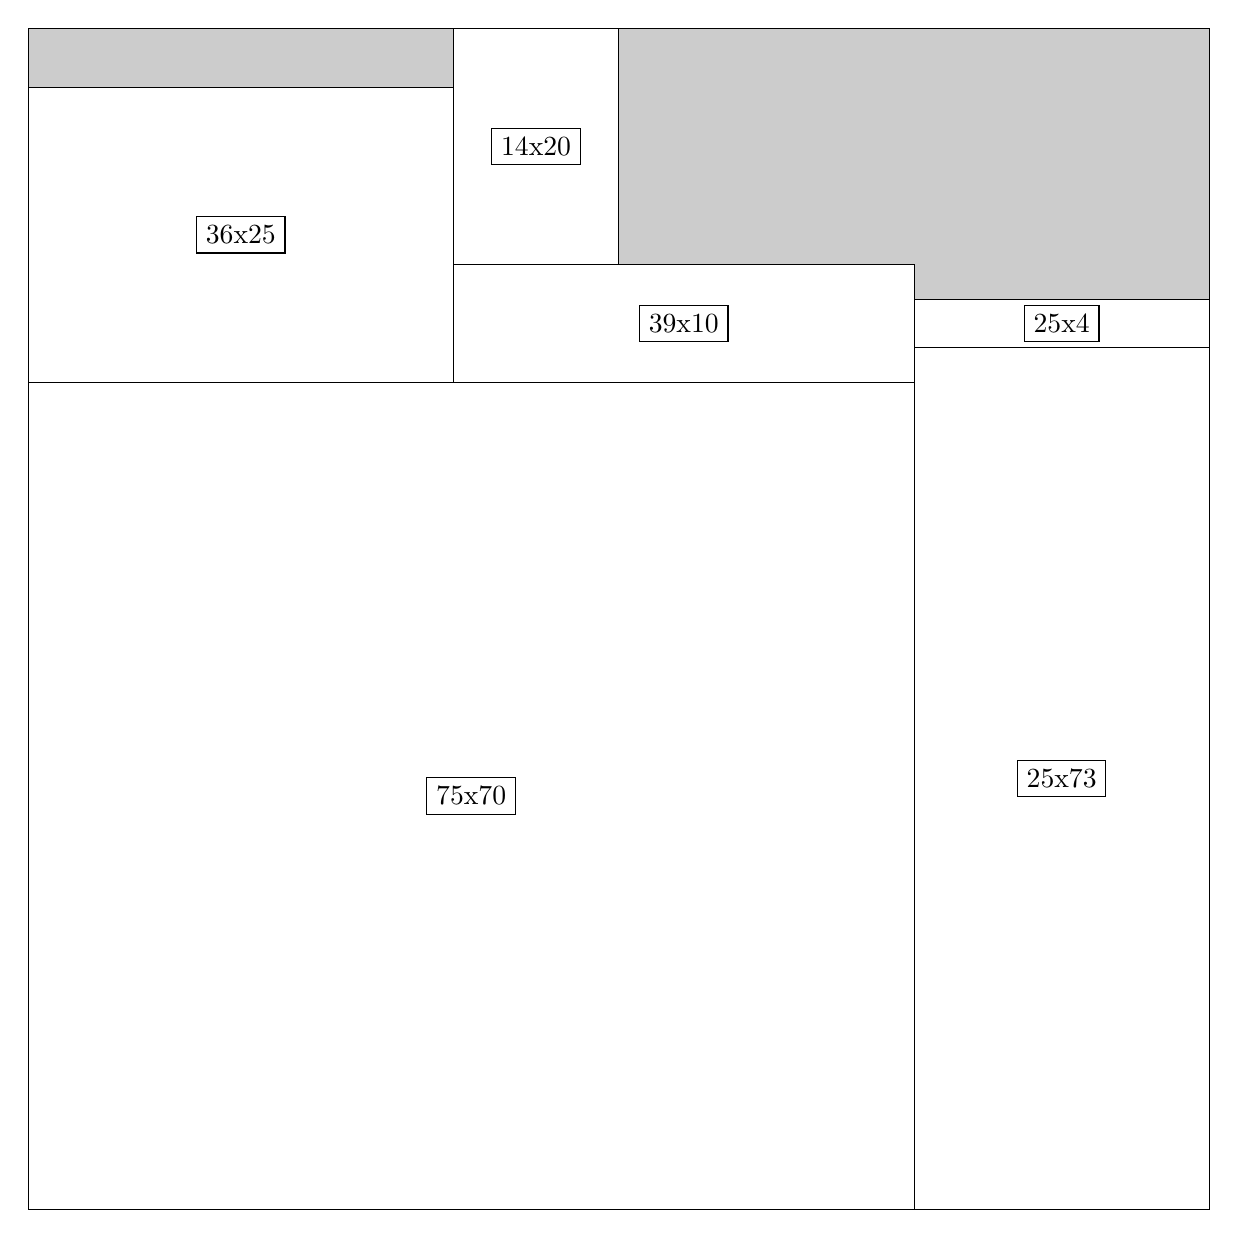
\begin{tikzpicture}[shorten >=1pt,scale=1.0,every node/.style={scale=1.0},->]
\tikzstyle{vertex}=[circle,fill=black!25,minimum size=14pt,inner sep=0pt]
\filldraw[fill=gray!40!white, draw=black] (0,0) rectangle (15.0,15.0);
\foreach \name/\x/\y/\w/\h in {75x70/0.0/0.0/11.25/10.5,25x73/11.25/0.0/3.75/10.95,36x25/0.0/10.5/5.3999999999999995/3.75,39x10/5.3999999999999995/10.5/5.85/1.5,14x20/5.3999999999999995/12.0/2.1/3.0,25x4/11.25/10.95/3.75/0.6}
\filldraw[fill=white!40!white, draw=black] (\x,\y) rectangle node[draw] (\name) {\name} ++(\w,\h);
\end{tikzpicture}


w =75 , h =70 , x =0 , y =0 , v =5250
\par
w =25 , h =73 , x =75 , y =0 , v =1825
\par
w =36 , h =25 , x =0 , y =70 , v =900
\par
w =39 , h =10 , x =36 , y =70 , v =390
\par
w =14 , h =20 , x =36 , y =80 , v =280
\par
w =25 , h =4 , x =75 , y =73 , v =100
\par
\newpage


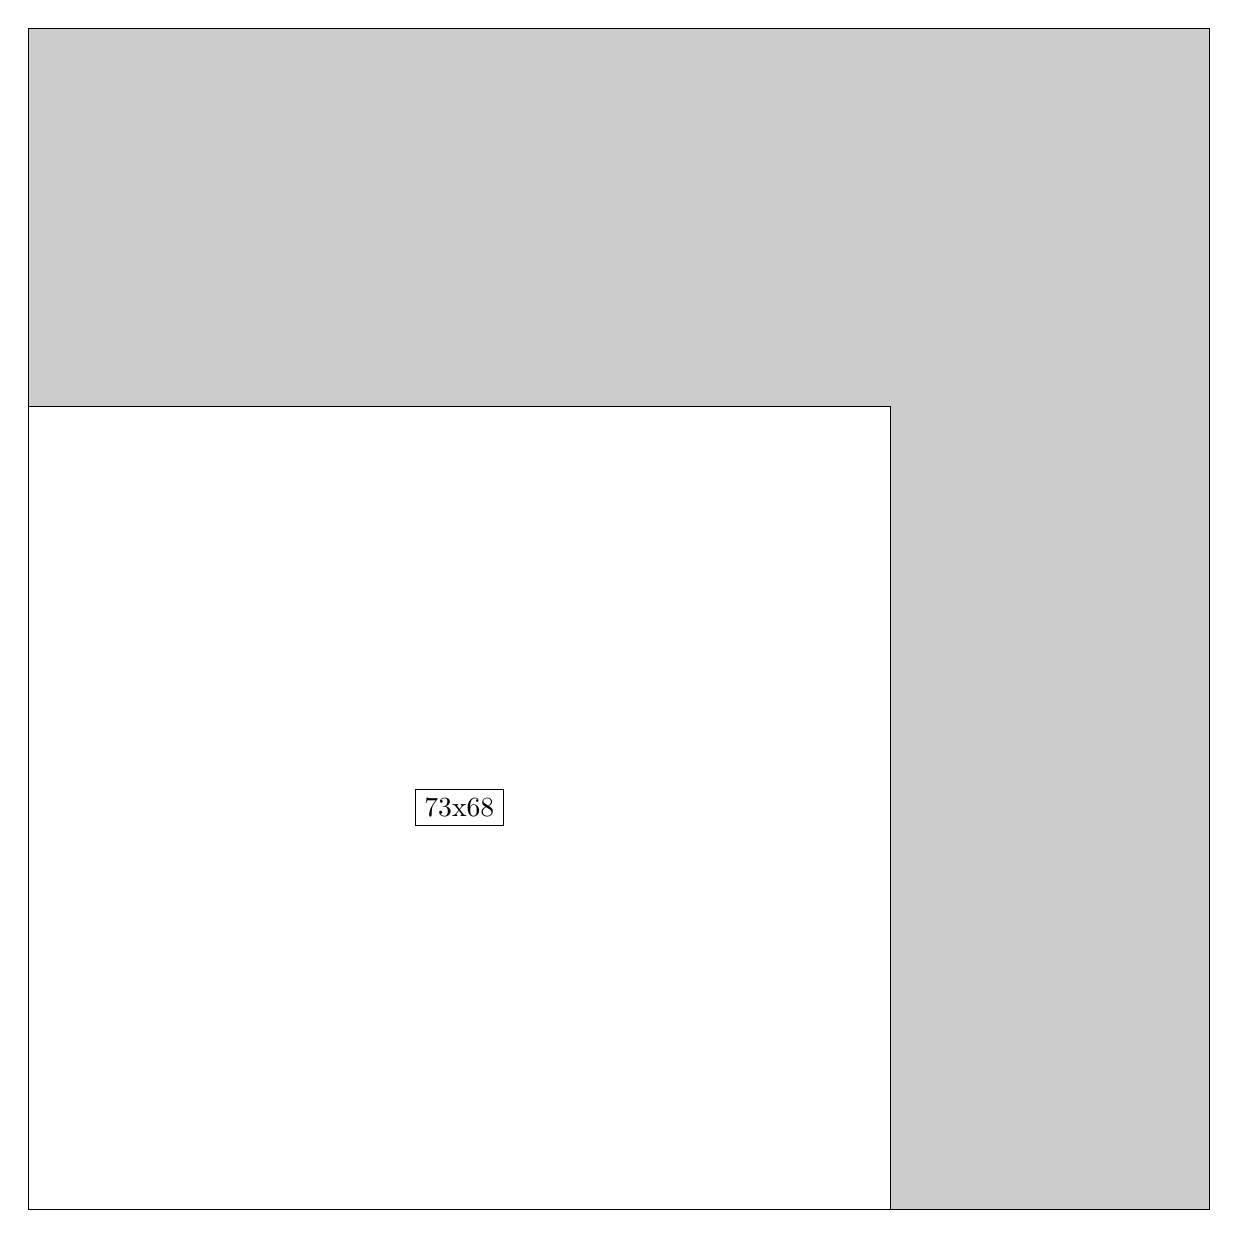
\begin{tikzpicture}[shorten >=1pt,scale=1.0,every node/.style={scale=1.0},->]
\tikzstyle{vertex}=[circle,fill=black!25,minimum size=14pt,inner sep=0pt]
\filldraw[fill=gray!40!white, draw=black] (0,0) rectangle (15.0,15.0);
\foreach \name/\x/\y/\w/\h in {73x68/0.0/0.0/10.95/10.2}
\filldraw[fill=white!40!white, draw=black] (\x,\y) rectangle node[draw] (\name) {\name} ++(\w,\h);
\end{tikzpicture}


w =73 , h =68 , x =0 , y =0 , v =4964
\par
\newpage


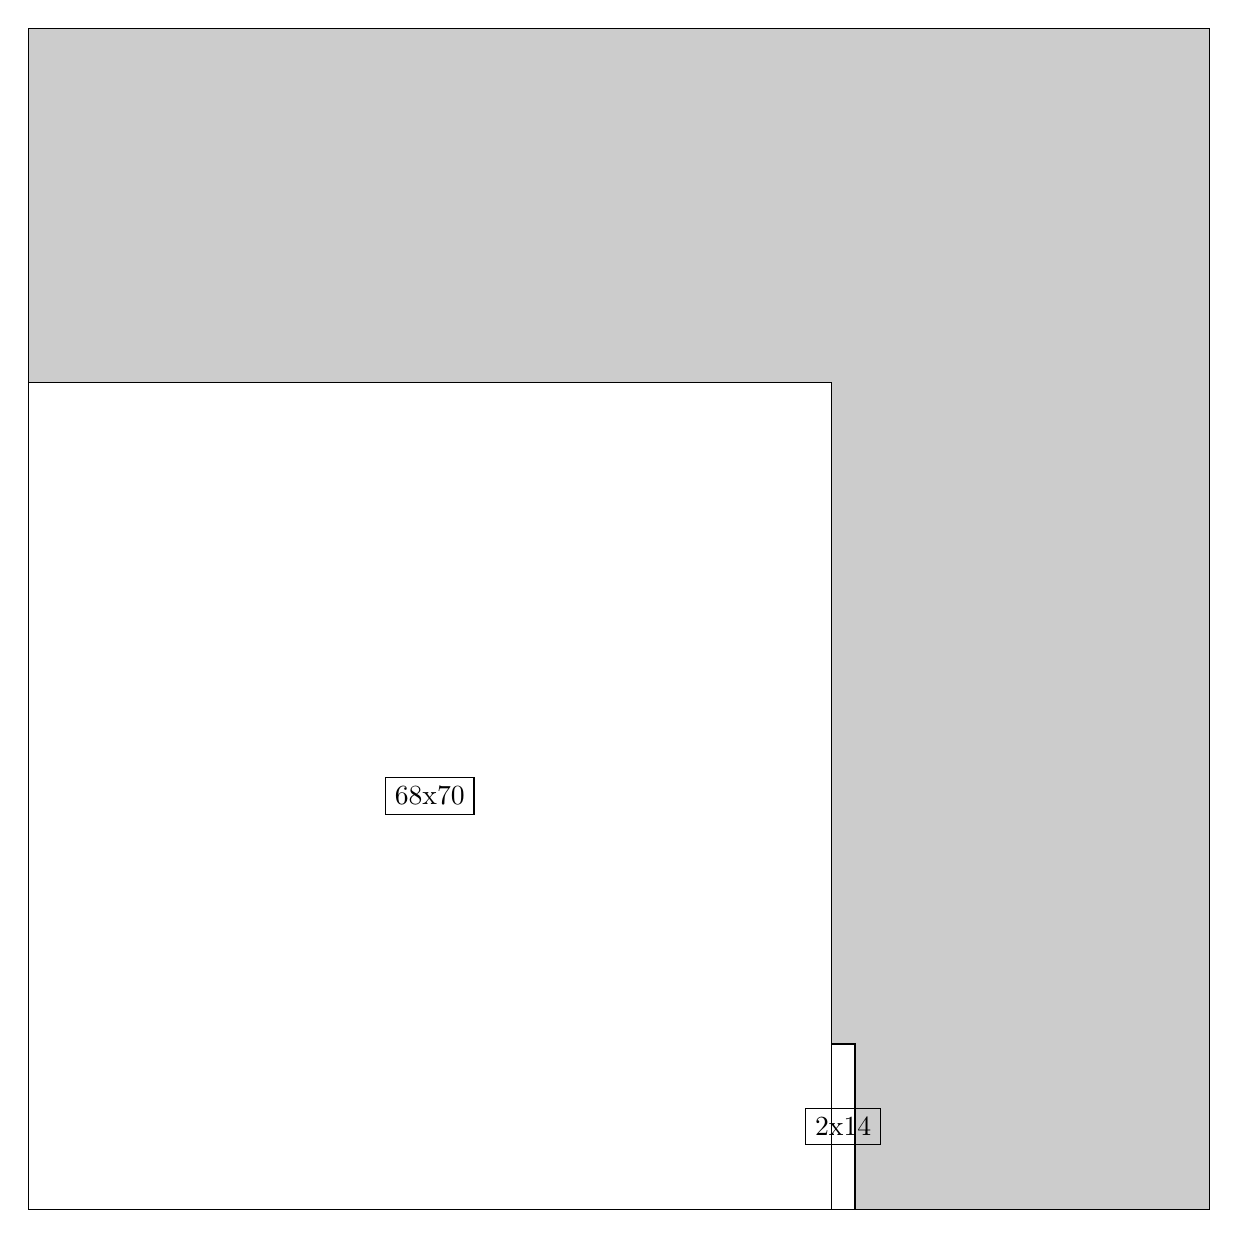
\begin{tikzpicture}[shorten >=1pt,scale=1.0,every node/.style={scale=1.0},->]
\tikzstyle{vertex}=[circle,fill=black!25,minimum size=14pt,inner sep=0pt]
\filldraw[fill=gray!40!white, draw=black] (0,0) rectangle (15.0,15.0);
\foreach \name/\x/\y/\w/\h in {68x70/0.0/0.0/10.2/10.5,2x14/10.2/0.0/0.3/2.1}
\filldraw[fill=white!40!white, draw=black] (\x,\y) rectangle node[draw] (\name) {\name} ++(\w,\h);
\end{tikzpicture}


w =68 , h =70 , x =0 , y =0 , v =4760
\par
w =2 , h =14 , x =68 , y =0 , v =28
\par
\newpage


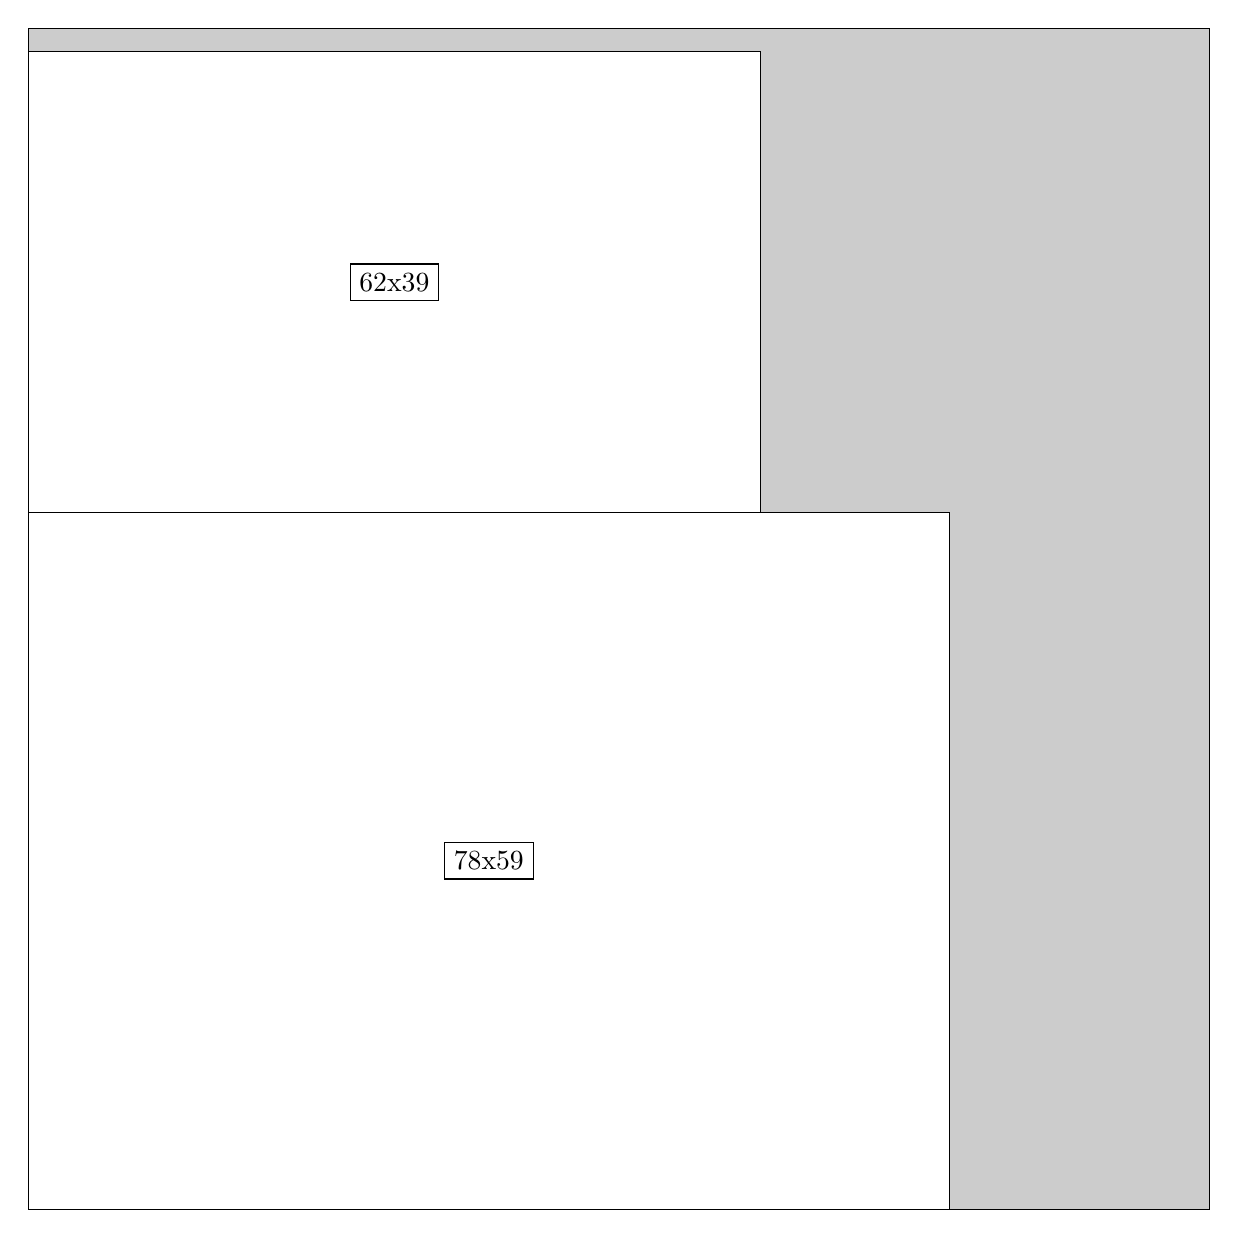
\begin{tikzpicture}[shorten >=1pt,scale=1.0,every node/.style={scale=1.0},->]
\tikzstyle{vertex}=[circle,fill=black!25,minimum size=14pt,inner sep=0pt]
\filldraw[fill=gray!40!white, draw=black] (0,0) rectangle (15.0,15.0);
\foreach \name/\x/\y/\w/\h in {78x59/0.0/0.0/11.7/8.85,62x39/0.0/8.85/9.299999999999999/5.85}
\filldraw[fill=white!40!white, draw=black] (\x,\y) rectangle node[draw] (\name) {\name} ++(\w,\h);
\end{tikzpicture}


w =78 , h =59 , x =0 , y =0 , v =4602
\par
w =62 , h =39 , x =0 , y =59 , v =2418
\par
\newpage


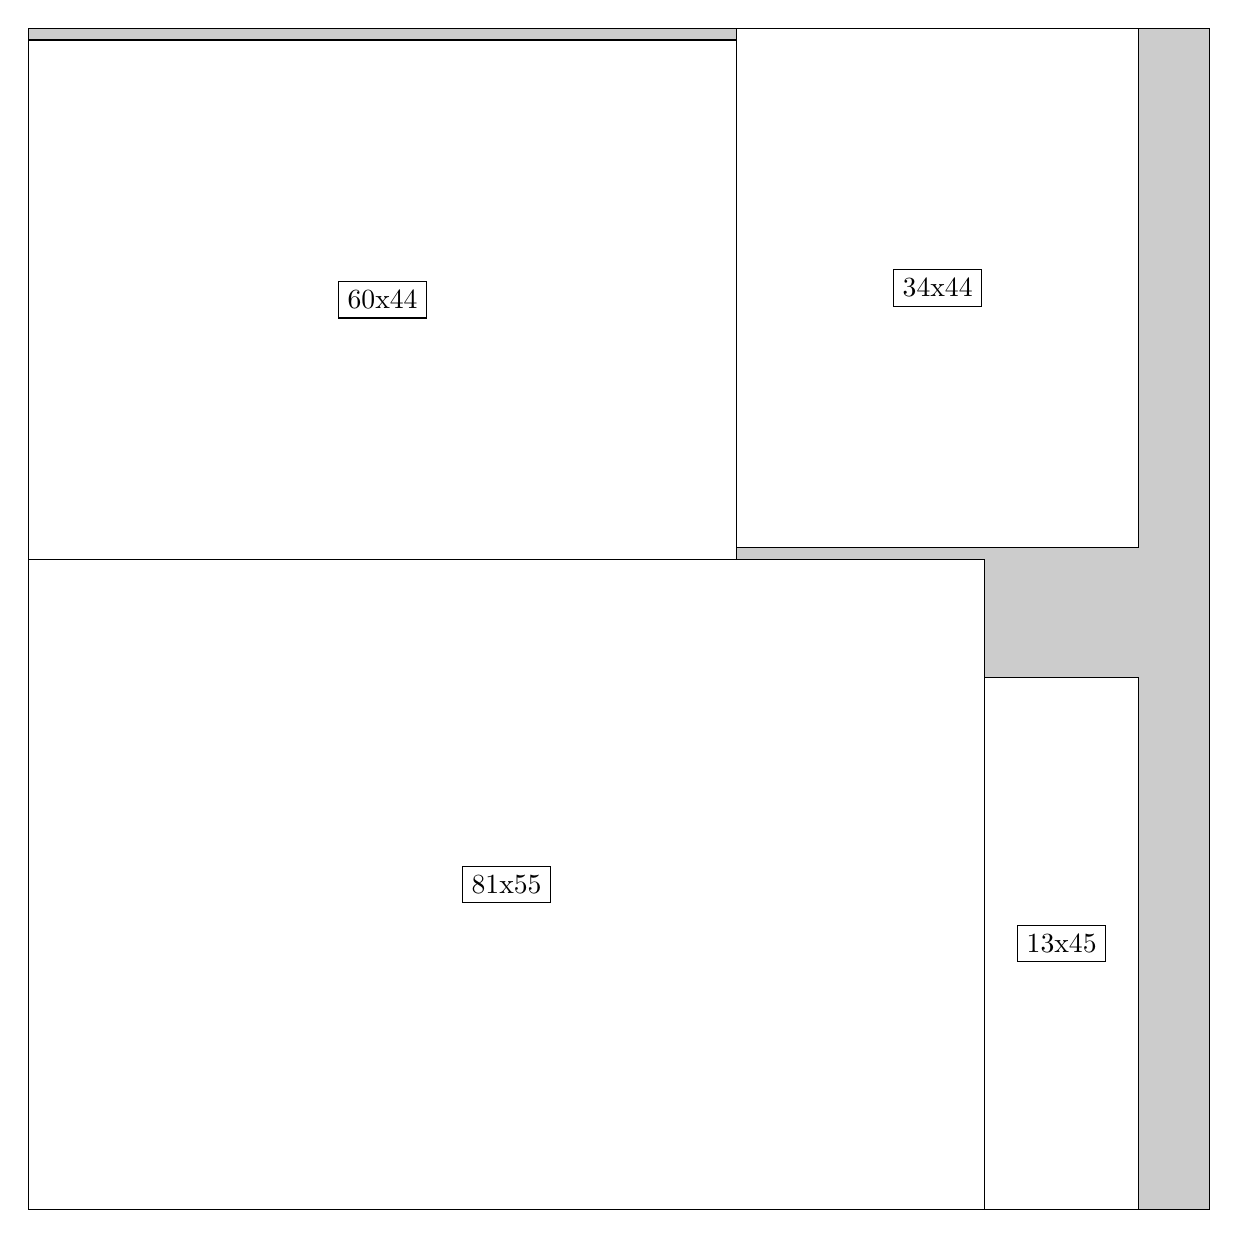
\begin{tikzpicture}[shorten >=1pt,scale=1.0,every node/.style={scale=1.0},->]
\tikzstyle{vertex}=[circle,fill=black!25,minimum size=14pt,inner sep=0pt]
\filldraw[fill=gray!40!white, draw=black] (0,0) rectangle (15.0,15.0);
\foreach \name/\x/\y/\w/\h in {81x55/0.0/0.0/12.15/8.25,60x44/0.0/8.25/9.0/6.6,34x44/9.0/8.4/5.1/6.6,13x45/12.15/0.0/1.95/6.75}
\filldraw[fill=white!40!white, draw=black] (\x,\y) rectangle node[draw] (\name) {\name} ++(\w,\h);
\end{tikzpicture}


w =81 , h =55 , x =0 , y =0 , v =4455
\par
w =60 , h =44 , x =0 , y =55 , v =2640
\par
w =34 , h =44 , x =60 , y =56 , v =1496
\par
w =13 , h =45 , x =81 , y =0 , v =585
\par
\newpage


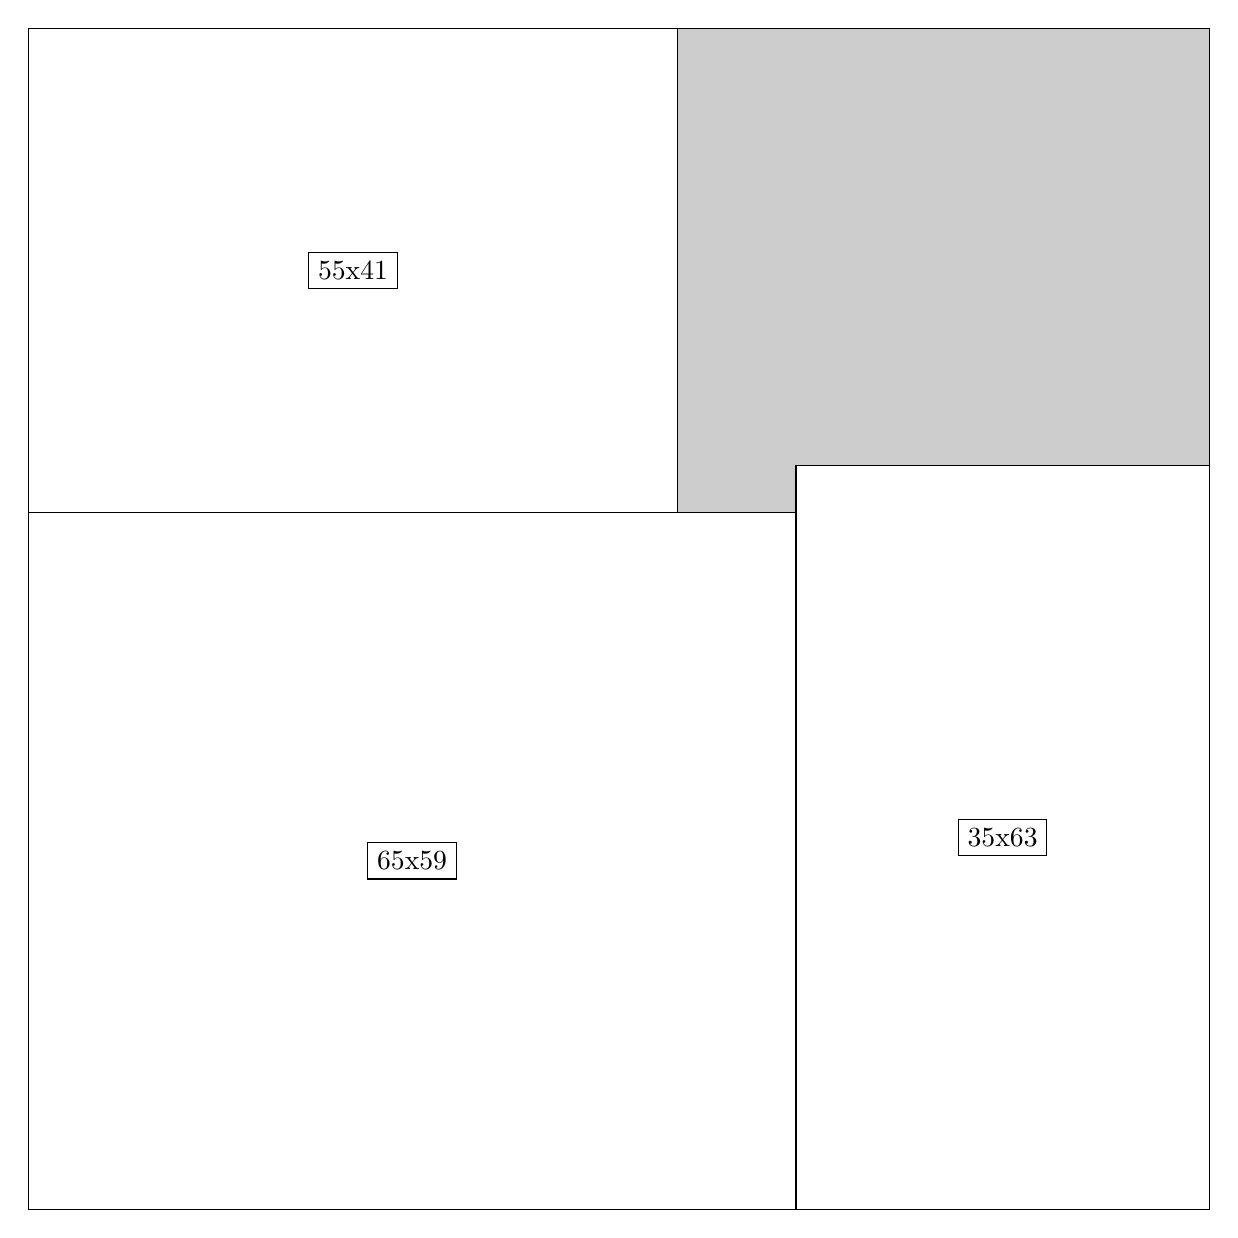
\begin{tikzpicture}[shorten >=1pt,scale=1.0,every node/.style={scale=1.0},->]
\tikzstyle{vertex}=[circle,fill=black!25,minimum size=14pt,inner sep=0pt]
\filldraw[fill=gray!40!white, draw=black] (0,0) rectangle (15.0,15.0);
\foreach \name/\x/\y/\w/\h in {65x59/0.0/0.0/9.75/8.85,55x41/0.0/8.85/8.25/6.1499999999999995,35x63/9.75/0.0/5.25/9.45}
\filldraw[fill=white!40!white, draw=black] (\x,\y) rectangle node[draw] (\name) {\name} ++(\w,\h);
\end{tikzpicture}


w =65 , h =59 , x =0 , y =0 , v =3835
\par
w =55 , h =41 , x =0 , y =59 , v =2255
\par
w =35 , h =63 , x =65 , y =0 , v =2205
\par
\newpage


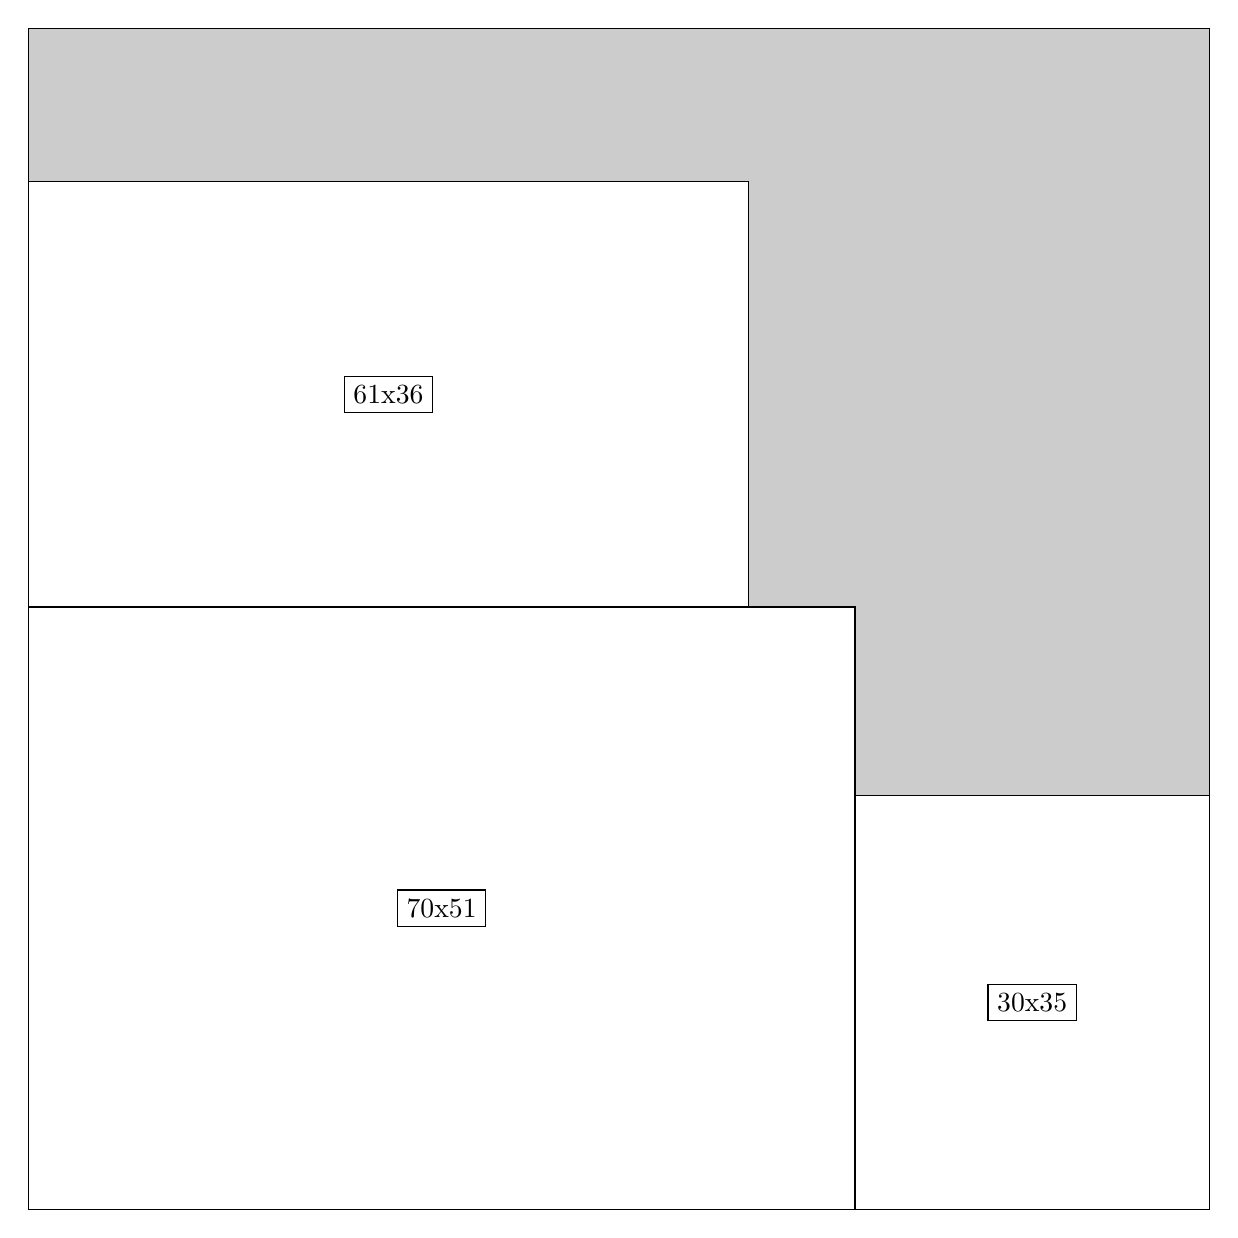
\begin{tikzpicture}[shorten >=1pt,scale=1.0,every node/.style={scale=1.0},->]
\tikzstyle{vertex}=[circle,fill=black!25,minimum size=14pt,inner sep=0pt]
\filldraw[fill=gray!40!white, draw=black] (0,0) rectangle (15.0,15.0);
\foreach \name/\x/\y/\w/\h in {70x51/0.0/0.0/10.5/7.6499999999999995,61x36/0.0/7.6499999999999995/9.15/5.3999999999999995,30x35/10.5/0.0/4.5/5.25}
\filldraw[fill=white!40!white, draw=black] (\x,\y) rectangle node[draw] (\name) {\name} ++(\w,\h);
\end{tikzpicture}


w =70 , h =51 , x =0 , y =0 , v =3570
\par
w =61 , h =36 , x =0 , y =51 , v =2196
\par
w =30 , h =35 , x =70 , y =0 , v =1050
\par
\newpage


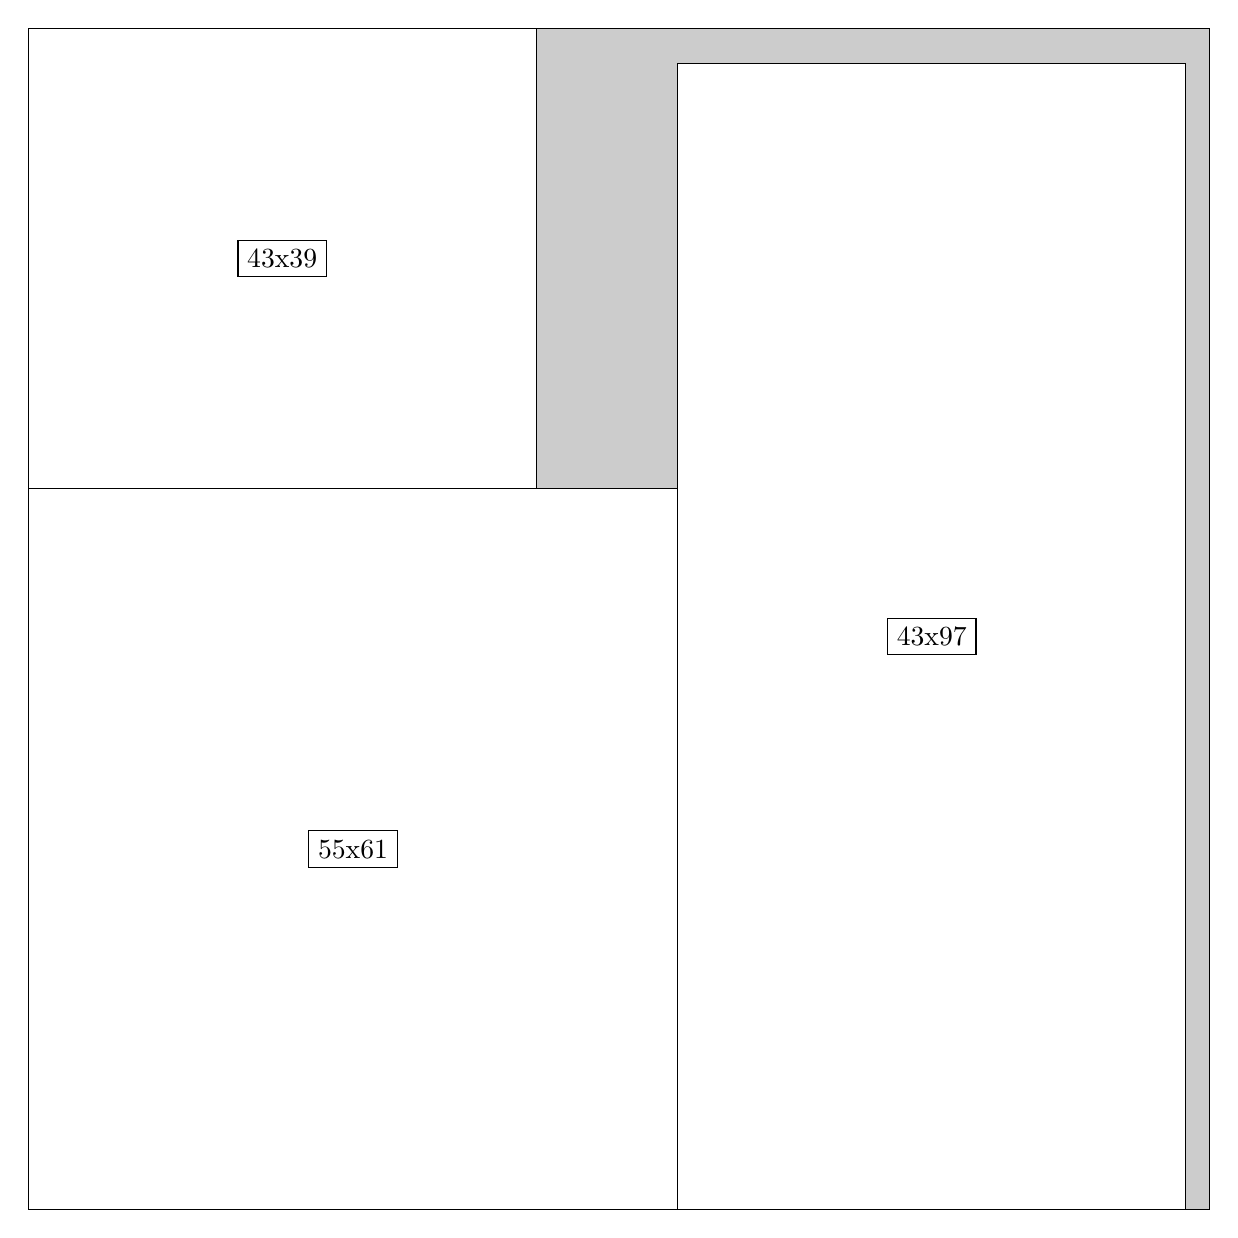
\begin{tikzpicture}[shorten >=1pt,scale=1.0,every node/.style={scale=1.0},->]
\tikzstyle{vertex}=[circle,fill=black!25,minimum size=14pt,inner sep=0pt]
\filldraw[fill=gray!40!white, draw=black] (0,0) rectangle (15.0,15.0);
\foreach \name/\x/\y/\w/\h in {43x97/8.25/0.0/6.45/14.549999999999999,55x61/0.0/0.0/8.25/9.15,43x39/0.0/9.15/6.45/5.85}
\filldraw[fill=white!40!white, draw=black] (\x,\y) rectangle node[draw] (\name) {\name} ++(\w,\h);
\end{tikzpicture}


w =43 , h =97 , x =55 , y =0 , v =4171
\par
w =55 , h =61 , x =0 , y =0 , v =3355
\par
w =43 , h =39 , x =0 , y =61 , v =1677
\par
\newpage


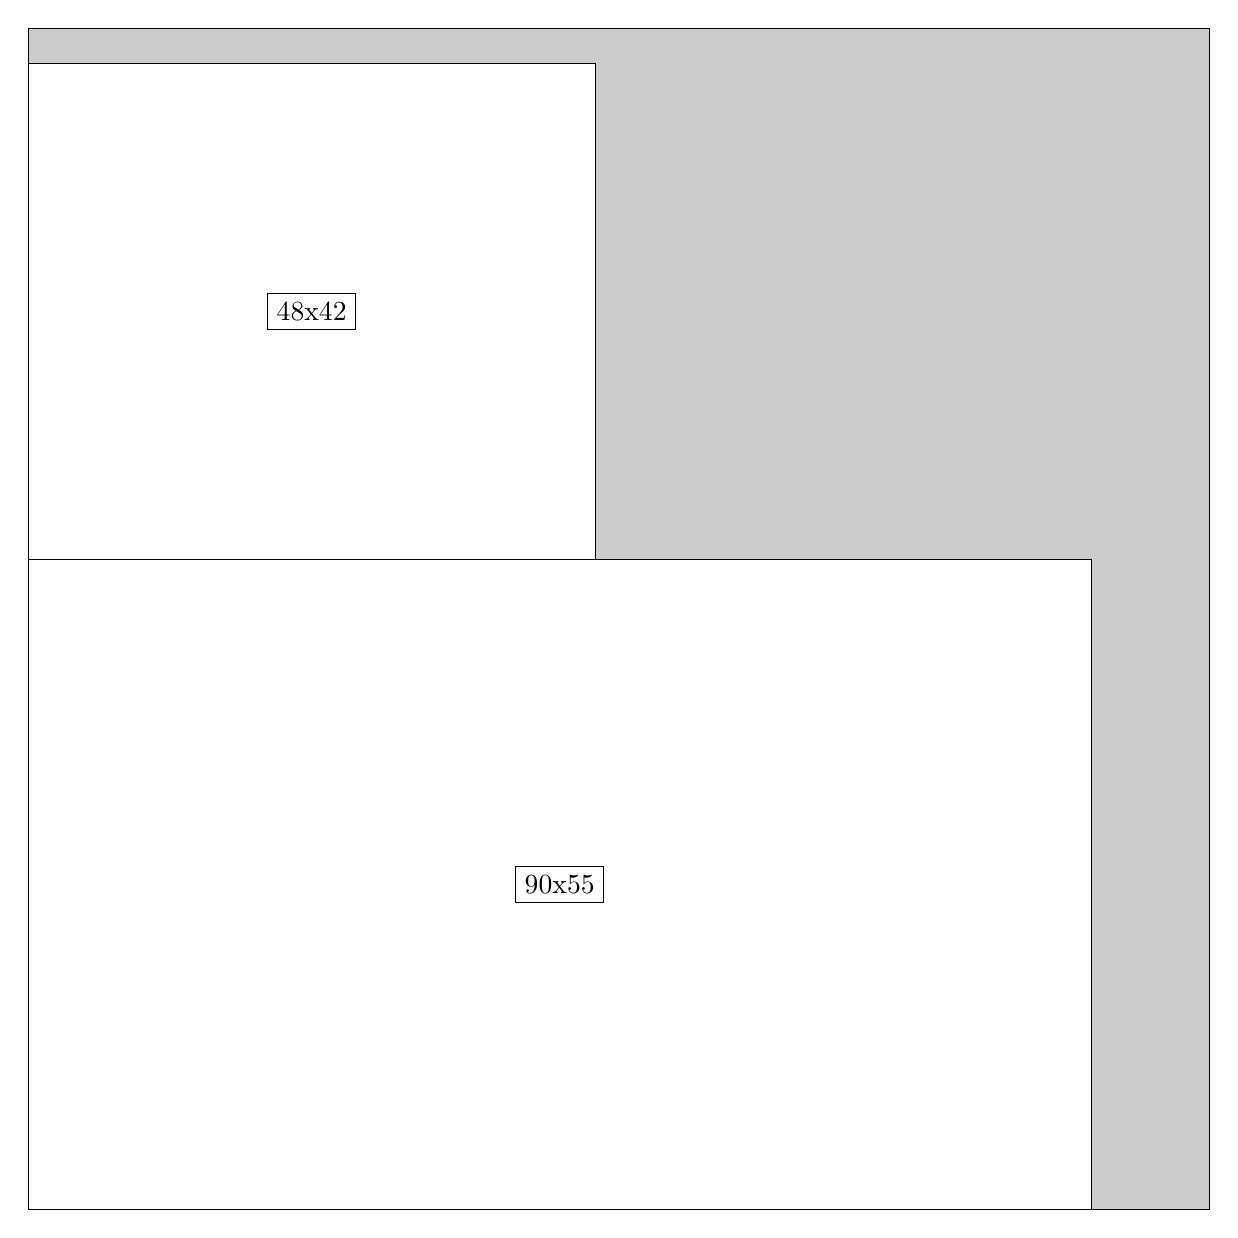
\begin{tikzpicture}[shorten >=1pt,scale=1.0,every node/.style={scale=1.0},->]
\tikzstyle{vertex}=[circle,fill=black!25,minimum size=14pt,inner sep=0pt]
\filldraw[fill=gray!40!white, draw=black] (0,0) rectangle (15.0,15.0);
\foreach \name/\x/\y/\w/\h in {90x55/0.0/0.0/13.5/8.25,48x42/0.0/8.25/7.199999999999999/6.3}
\filldraw[fill=white!40!white, draw=black] (\x,\y) rectangle node[draw] (\name) {\name} ++(\w,\h);
\end{tikzpicture}


w =90 , h =55 , x =0 , y =0 , v =4950
\par
w =48 , h =42 , x =0 , y =55 , v =2016
\par
\newpage


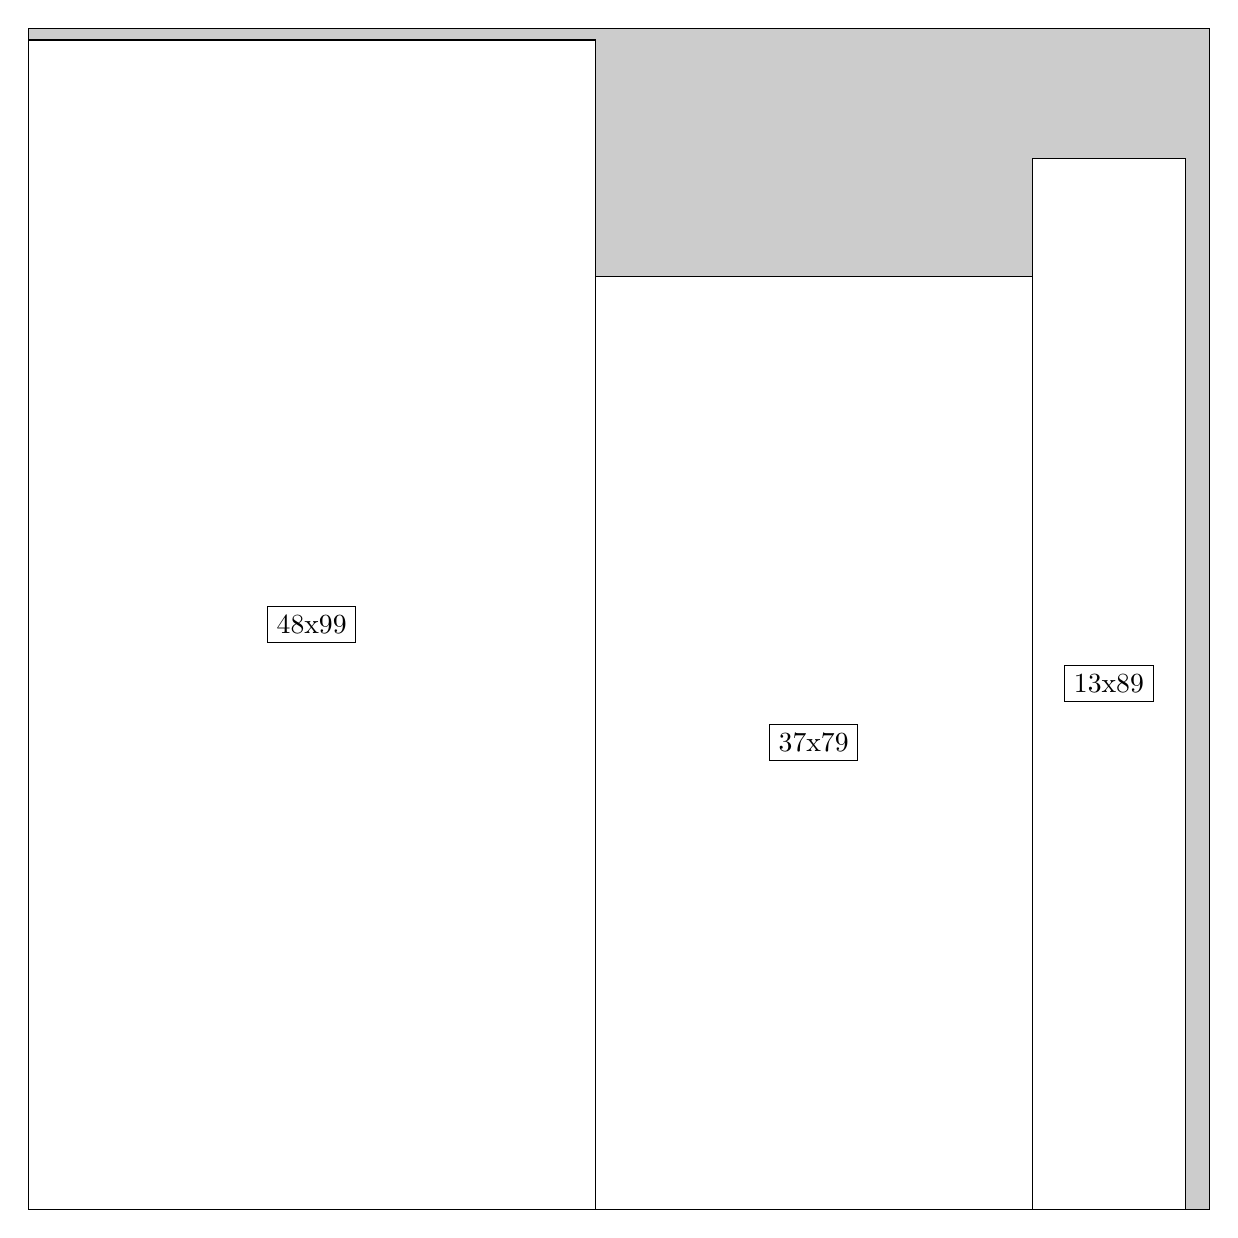
\begin{tikzpicture}[shorten >=1pt,scale=1.0,every node/.style={scale=1.0},->]
\tikzstyle{vertex}=[circle,fill=black!25,minimum size=14pt,inner sep=0pt]
\filldraw[fill=gray!40!white, draw=black] (0,0) rectangle (15.0,15.0);
\foreach \name/\x/\y/\w/\h in {48x99/0.0/0.0/7.199999999999999/14.85,37x79/7.199999999999999/0.0/5.55/11.85,13x89/12.75/0.0/1.95/13.35}
\filldraw[fill=white!40!white, draw=black] (\x,\y) rectangle node[draw] (\name) {\name} ++(\w,\h);
\end{tikzpicture}


w =48 , h =99 , x =0 , y =0 , v =4752
\par
w =37 , h =79 , x =48 , y =0 , v =2923
\par
w =13 , h =89 , x =85 , y =0 , v =1157
\par
\newpage


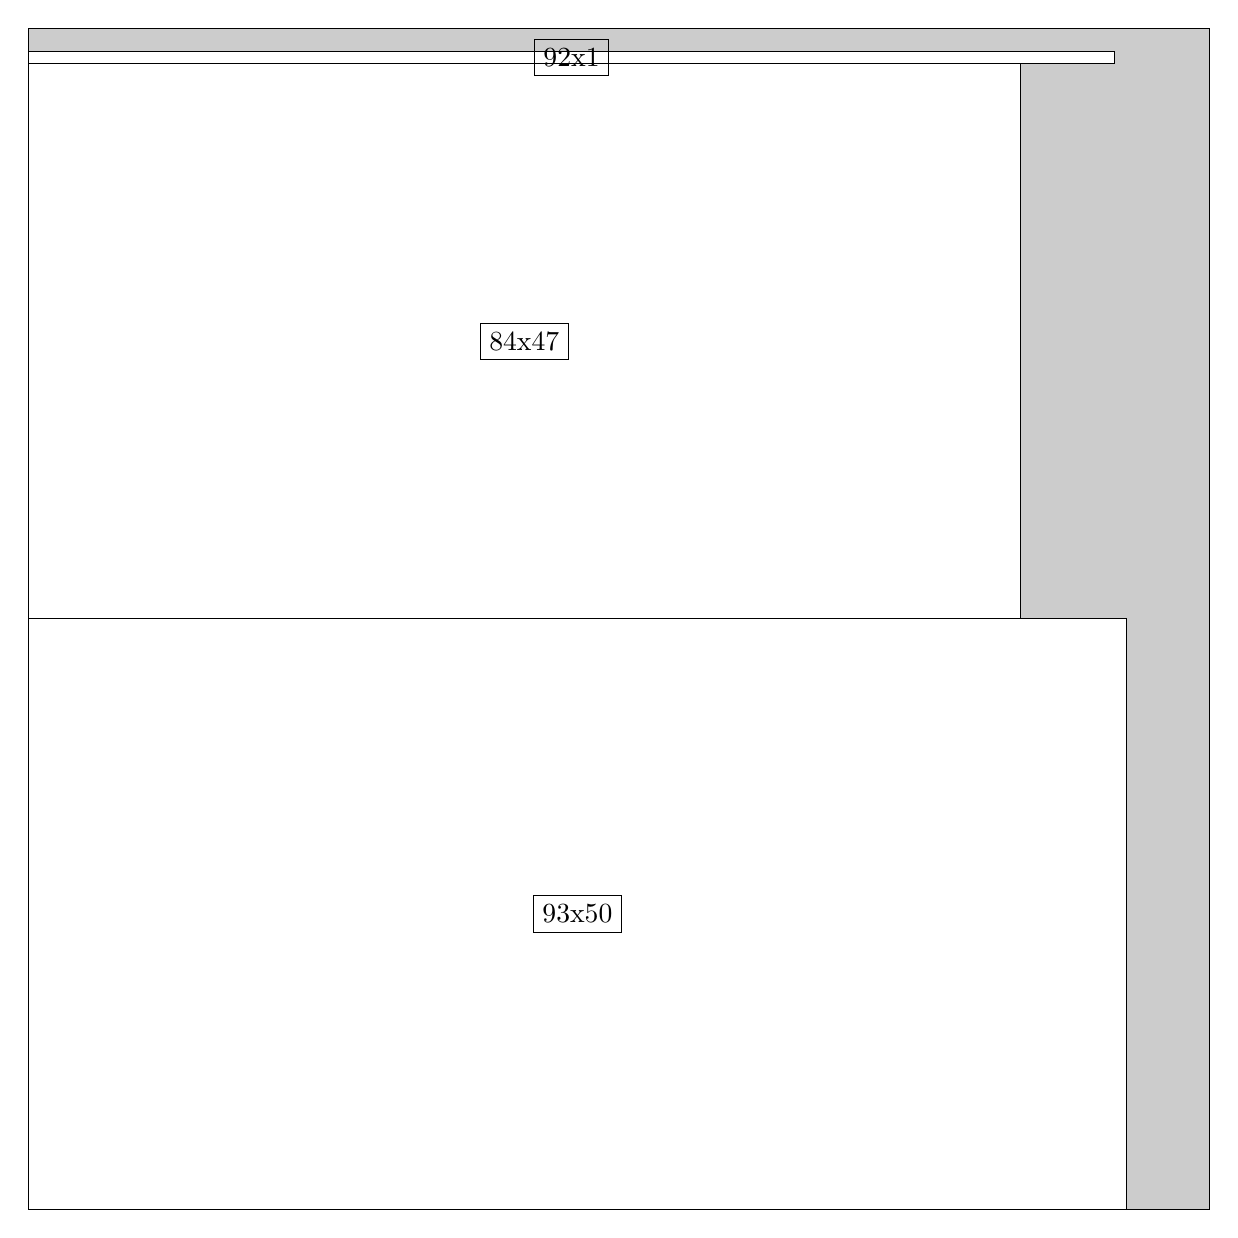
\begin{tikzpicture}[shorten >=1pt,scale=1.0,every node/.style={scale=1.0},->]
\tikzstyle{vertex}=[circle,fill=black!25,minimum size=14pt,inner sep=0pt]
\filldraw[fill=gray!40!white, draw=black] (0,0) rectangle (15.0,15.0);
\foreach \name/\x/\y/\w/\h in {93x50/0.0/0.0/13.95/7.5,84x47/0.0/7.5/12.6/7.05,92x1/0.0/14.549999999999999/13.799999999999999/0.15}
\filldraw[fill=white!40!white, draw=black] (\x,\y) rectangle node[draw] (\name) {\name} ++(\w,\h);
\end{tikzpicture}


w =93 , h =50 , x =0 , y =0 , v =4650
\par
w =84 , h =47 , x =0 , y =50 , v =3948
\par
w =92 , h =1 , x =0 , y =97 , v =92
\par
\newpage


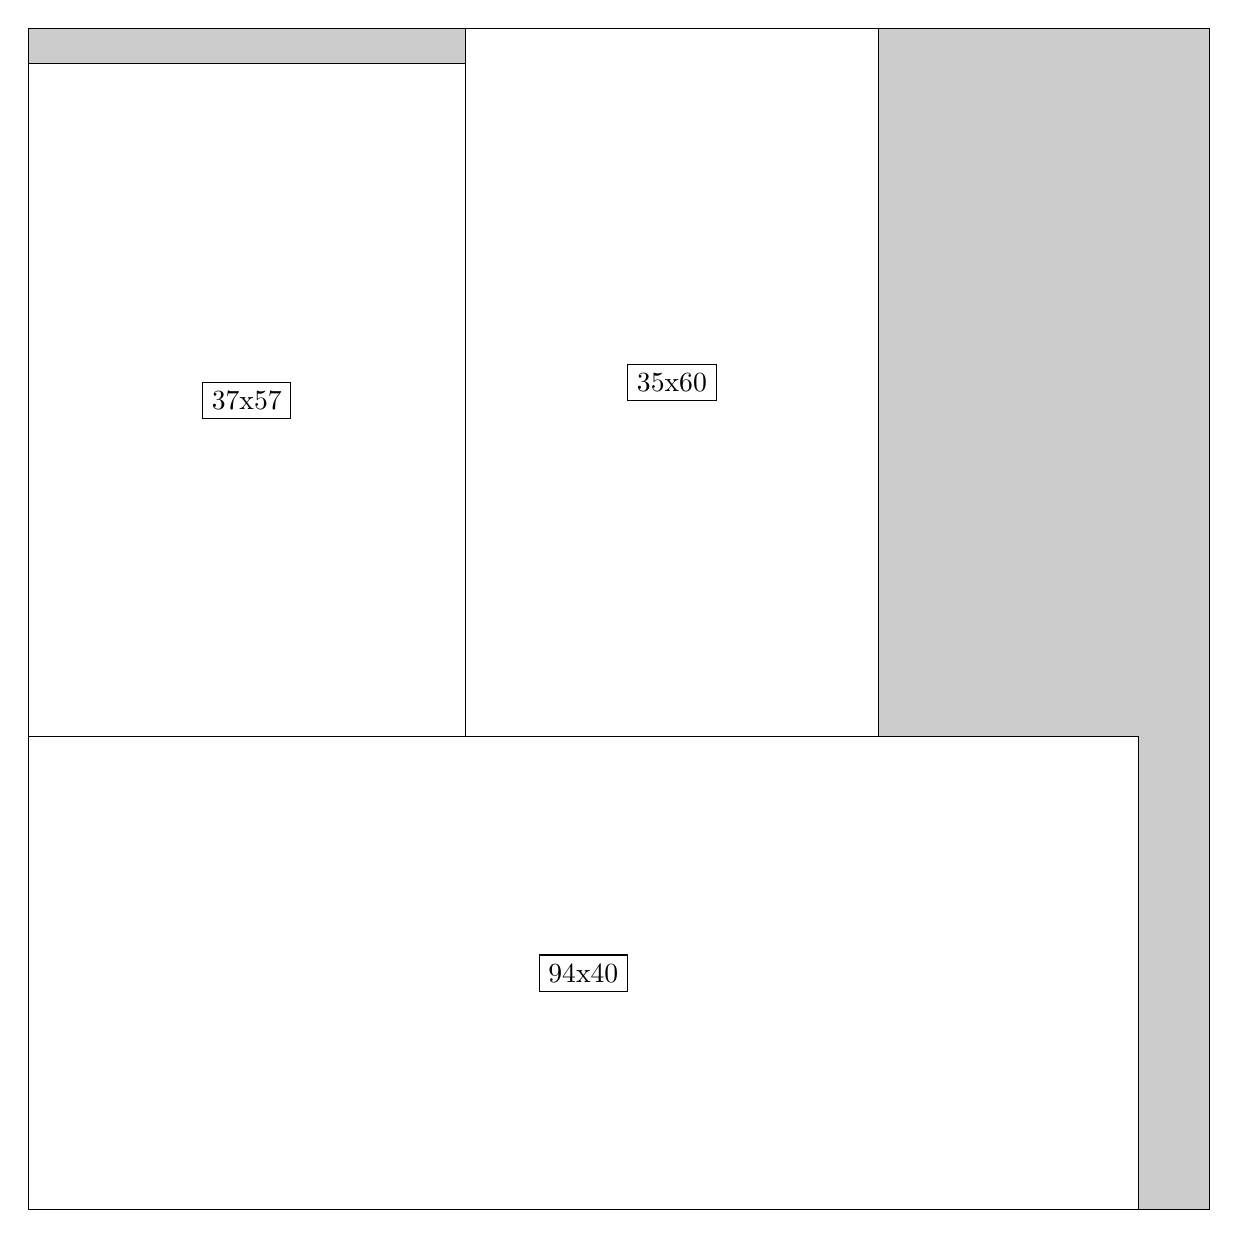
\begin{tikzpicture}[shorten >=1pt,scale=1.0,every node/.style={scale=1.0},->]
\tikzstyle{vertex}=[circle,fill=black!25,minimum size=14pt,inner sep=0pt]
\filldraw[fill=gray!40!white, draw=black] (0,0) rectangle (15.0,15.0);
\foreach \name/\x/\y/\w/\h in {94x40/0.0/0.0/14.1/6.0,37x57/0.0/6.0/5.55/8.549999999999999,35x60/5.55/6.0/5.25/9.0}
\filldraw[fill=white!40!white, draw=black] (\x,\y) rectangle node[draw] (\name) {\name} ++(\w,\h);
\end{tikzpicture}


w =94 , h =40 , x =0 , y =0 , v =3760
\par
w =37 , h =57 , x =0 , y =40 , v =2109
\par
w =35 , h =60 , x =37 , y =40 , v =2100
\par
\newpage


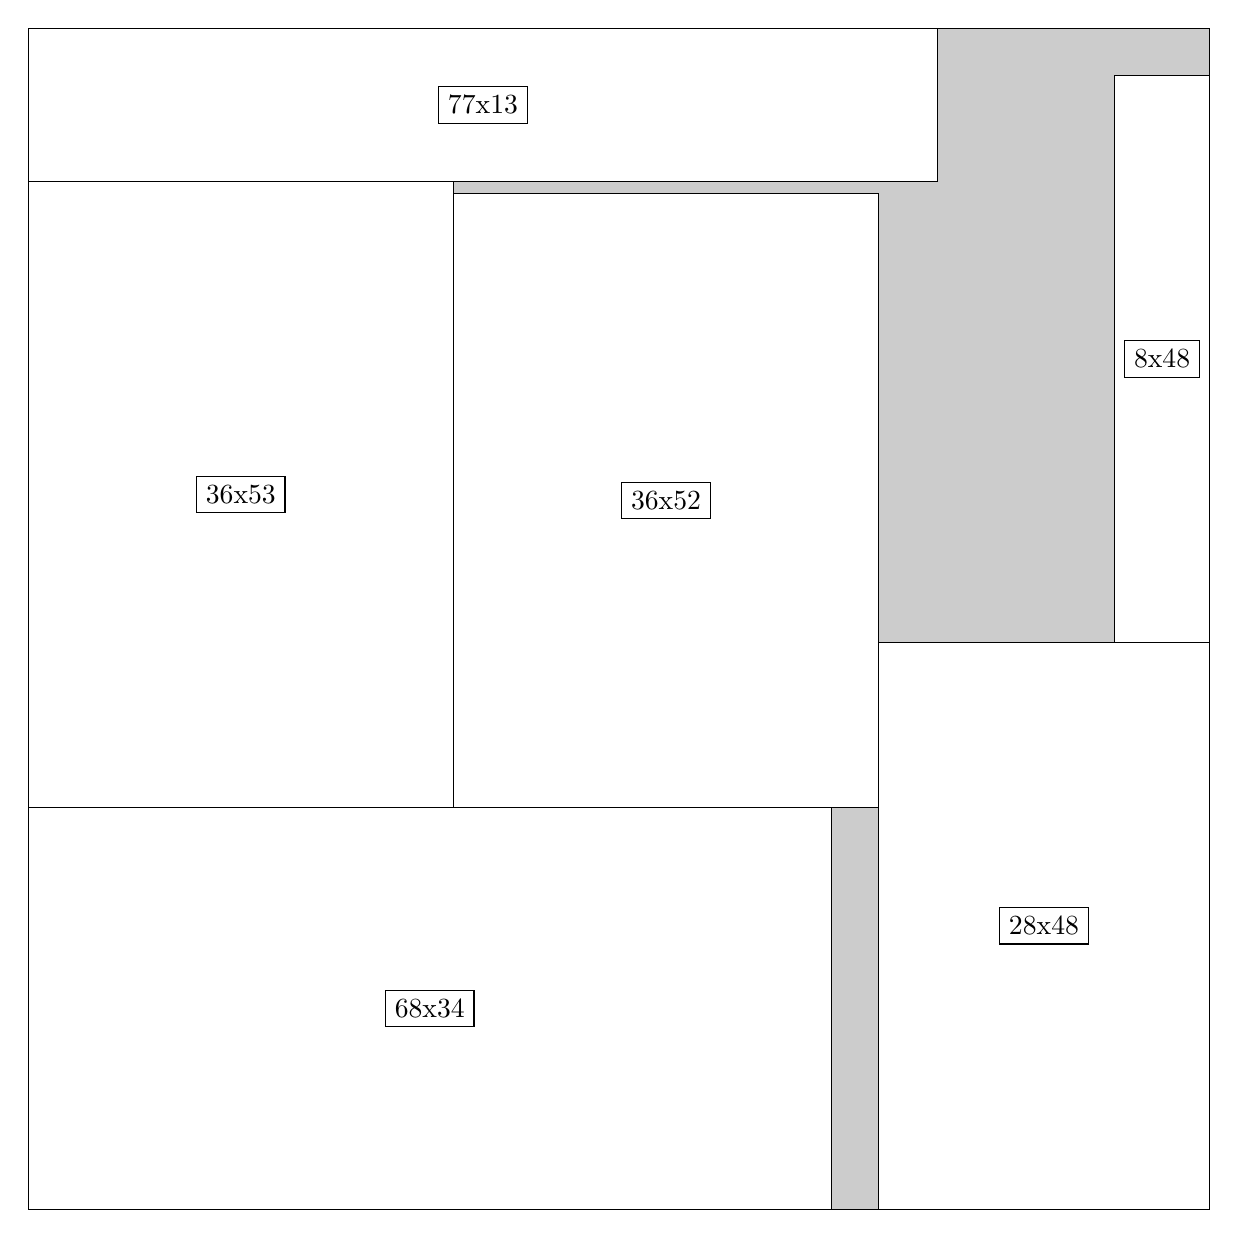
\begin{tikzpicture}[shorten >=1pt,scale=1.0,every node/.style={scale=1.0},->]
\tikzstyle{vertex}=[circle,fill=black!25,minimum size=14pt,inner sep=0pt]
\filldraw[fill=gray!40!white, draw=black] (0,0) rectangle (15.0,15.0);
\foreach \name/\x/\y/\w/\h in {68x34/0.0/0.0/10.2/5.1,36x53/0.0/5.1/5.3999999999999995/7.949999999999999,36x52/5.3999999999999995/5.1/5.3999999999999995/7.8,77x13/0.0/13.049999999999999/11.549999999999999/1.95,8x48/13.799999999999999/7.199999999999999/1.2/7.199999999999999,28x48/10.799999999999999/0.0/4.2/7.199999999999999}
\filldraw[fill=white!40!white, draw=black] (\x,\y) rectangle node[draw] (\name) {\name} ++(\w,\h);
\end{tikzpicture}


w =68 , h =34 , x =0 , y =0 , v =2312
\par
w =36 , h =53 , x =0 , y =34 , v =1908
\par
w =36 , h =52 , x =36 , y =34 , v =1872
\par
w =77 , h =13 , x =0 , y =87 , v =1001
\par
w =8 , h =48 , x =92 , y =48 , v =384
\par
w =28 , h =48 , x =72 , y =0 , v =1344
\par
\newpage


\end{document}